\documentclass[aspectratio=169,11pt]{ctexbeamer}
\usepackage{amsmath,amssymb,mathtools,bm}
\usepackage{hyperref}
\usepackage{graphicx}
\usepackage{booktabs}
\usepackage{tikz}
\usetikzlibrary{arrows.meta,positioning,calc}

\usetheme{Madrid}
\usecolortheme{default}
\setbeamertemplate{navigation symbols}{}

\definecolor{MainBlue}{RGB}{25,70,140}
\definecolor{Accent}{RGB}{180,60,40}

\newcommand{\e}{\mathrm{e}}
\newcommand{\R}{\mathbb{R}}
\newcommand{\dx}{\,\mathrm{d}x}
\newcommand{\dy}{\,\mathrm{d}y}

% Unified Yingxing Beamer footer and visual style.
\newcommand{\huayinglogo}{assets/logo1.jpg}
\newcommand{\huayingslogan}{英行培优，成绩无忧；英行相伴，刮目相看}

\setbeamersize{text margin left=8mm,text margin right=8mm}
\setbeamerfont{frametitle}{size=\large}
\setbeamercolor{structure}{fg=blue!70!black}
\setbeamercolor{frametitle}{bg=blue!75!black,fg=white}
\setbeamercolor{block title}{bg=blue!10,fg=black}
\setbeamercolor{block body}{bg=blue!2,fg=black}
\setbeamercolor{author in head/foot}{bg=blue!8,fg=black}
\setbeamercolor{title in head/foot}{bg=blue!8,fg=black}

\setbeamertemplate{footline}{%
  \leavevmode%
  \hbox{%
    \begin{beamercolorbox}[wd=.12\paperwidth,ht=3.8ex,dp=1.2ex,center]{author in head/foot}%
      \includegraphics[height=2.9ex]{\huayinglogo}%
    \end{beamercolorbox}%
    \begin{beamercolorbox}[wd=.76\paperwidth,ht=3.8ex,dp=1.2ex,center]{title in head/foot}%
      \scriptsize \huayingslogan
    \end{beamercolorbox}%
    \begin{beamercolorbox}[wd=.12\paperwidth,ht=3.8ex,dp=1.2ex,right]{author in head/foot}%
      \scriptsize \insertframenumber/\inserttotalframenumber\hspace*{1em}
    \end{beamercolorbox}%
  }%
}

\title{第四章 微分及其逆运算}
\subtitle{导数、可微与求导法则}
\author{数学讲义整理}
\date{}

\begin{document}

\begin{frame}
  \titlepage
\end{frame}

\begin{frame}{本节结构}
\begin{center}
\begin{tikzpicture}[>=Latex,node distance=1.55cm]
  \node[draw,rounded corners,fill=blue!8,minimum width=3.2cm,minimum height=0.95cm] (c1) {核心概念};
  \node[draw,rounded corners,fill=blue!8,minimum width=3.2cm,minimum height=0.95cm,right=of c1] (c2) {基本关系};
  \node[draw,rounded corners,fill=blue!8,minimum width=3.2cm,minimum height=0.95cm,right=of c2] (c3) {几何与应用};
  \node[draw,rounded corners,fill=blue!8,minimum width=3.2cm,minimum height=0.95cm,below=1.2cm of c2] (c4) {运算法则};
  \node[draw,rounded corners,fill=blue!8,minimum width=3.2cm,minimum height=0.95cm,left=of c4] (c5) {常用公式与微分};
  \node[draw,rounded corners,fill=blue!8,minimum width=3.2cm,minimum height=0.95cm,right=of c4] (c6) {例题与练习};
  \draw[->,thick] (c1) -- (c2);
  \draw[->,thick] (c2) -- (c3);
  \draw[->,thick] (c2) -- (c4);
  \draw[->,thick] (c4) -- (c5);
  \draw[->,thick] (c4) -- (c6);
  \node[below=2.25cm of c4,align=center] {\small 先建立概念，再梳理关系，随后进入几何直观与运算，最后用例题和练习巩固。};
\end{tikzpicture}
\end{center}
\end{frame}

\section{核心概念}

\begin{frame}{导数的定义}
设函数 $f$ 在 $x_0$ 附近有定义，若极限
\[
\lim_{x\to x_0}\frac{f(x)-f(x_0)}{x-x_0}
\]
存在且有限，则称 $f$ 在 $x_0$ 处\alert{可导}，并把该极限记作
\[
f'(x_0).
\]

\vspace{0.6em}
若记 $\Delta x=x-x_0,\ \Delta y=f(x)-f(x_0)$，则
\[
f'(x_0)=\lim_{\Delta x\to 0}\frac{\Delta y}{\Delta x}.
\]
\end{frame}

\begin{frame}{左右导数与可导判定}
\[
f'_-(x_0)=\lim_{x\to x_0^-}\frac{f(x)-f(x_0)}{x-x_0},
\qquad
f'_+(x_0)=\lim_{x\to x_0^+}\frac{f(x)-f(x_0)}{x-x_0}.
\]

\begin{block}{判定}
$f$ 在 $x_0$ 处可导，当且仅当左右导数都存在且相等，即
\[
f'_-(x_0)=f'_+(x_0).
\]
\end{block}

\begin{alertblock}{常见失分点}
连续不一定可导，例如 $f(x)=|x|$ 在 $x=0$ 处连续但不可导。
\end{alertblock}
\end{frame}

\begin{frame}{左右导数可视化}
\begin{center}
\begin{tikzpicture}[scale=1.0,>=Latex]
  \draw[->] (-3.2,0) -- (3.2,0) node[right] {$x$};
  \draw[->] (0,-0.2) -- (0,3.1) node[above] {$y$};
  \draw[thick,MainBlue] (-2.6,2.6) -- (0,0) -- (2.6,2.6);
  \fill (0,0) circle (2pt) node[below left] {$O$};
  \draw[Accent,thick] (-1.9,1.9) -- (0,0) node[midway,above left] {\small 左斜率 $-1$};
  \draw[Accent,thick] (0,0) -- (1.9,1.9) node[midway,above right] {\small 右斜率 $1$};
  \node[align=center] at (0,2.65) {\small $f(x)=|x|$ 在 $x=0$ 处\\[-0.1em]\small 左右导数不相等};
\end{tikzpicture}
\end{center}
\end{frame}

\begin{frame}{可微的定义}
若存在常数 $A$，使得
\[
f(x)=f(x_0)+A(x-x_0)+o(x-x_0)\qquad (x\to x_0),
\]
则称 $f$ 在 $x_0$ 处\alert{可微}。

\begin{block}{微分表达}
\[
\mathrm{d}f(x_0)=f'(x_0)\,\mathrm{d}x(x_0).
\]
\end{block}
\end{frame}

\section{基本关系}

\begin{frame}{可导与可微的关系}
\small
\textbf{结论：}
\[
f \text{ 在 } x_0 \text{ 处可导}
\Longleftrightarrow
f \text{ 在 } x_0 \text{ 处可微}.
\]
并且当可微时，线性主部的系数就是导数：
\[
A=f'(x_0).
\]

\vspace{0.5em}
\begin{block}{同时要记住}
\[
\text{可导} \Longrightarrow \text{连续},
\qquad
\text{连续不推出可导}.
\]
\end{block}
\end{frame}

\begin{frame}{关系图}
\begin{center}
\begin{tikzpicture}[>=Latex,node distance=1.9cm]
  \node[draw,rounded corners,fill=blue!8,minimum width=2.8cm,minimum height=1cm] (d1) {可导};
  \node[draw,rounded corners,fill=blue!8,minimum width=2.8cm,minimum height=1cm,right=of d1] (d2) {可微};
  \node[draw,rounded corners,fill=blue!8,minimum width=2.8cm,minimum height=1cm,right=of d2] (d3) {连续};
  \draw[->,thick] (d1) -- (d2);
  \draw[->,thick] (d2) -- (d3);
  \node[below=1.2cm of d2,draw,rounded corners,fill=red!6,minimum width=4.6cm,minimum height=1cm] (counter) {$|x|$ 在 $x=0$ 连续但不可导};
  \draw[->,thick,Accent] ($(d3.south)+(0.55,0)$) .. controls +(0,-0.8) and +(0,0.8) .. ($(counter.north)+(1.2,0)$);
\end{tikzpicture}
\end{center}
\end{frame}

\begin{frame}{可导等价于可微的证明}
\small
\textbf{答案：}

\textbf{(1)} 若 $f$ 在 $x_0$ 处可导，则
\[
\lim_{x\to x_0}\frac{f(x)-f(x_0)-f'(x_0)(x-x_0)}{x-x_0}
=\lim_{x\to x_0}\frac{f(x)-f(x_0)}{x-x_0}-f'(x_0)=0.
\]
因此
\[
f(x)-f(x_0)-f'(x_0)(x-x_0)=o(x-x_0),
\]
即
\[
f(x)=f(x_0)+f'(x_0)(x-x_0)+o(x-x_0),
\]
这说明 $f$ 在 $x_0$ 处可微。

\vspace{0.4em}
反之，若
\[
f(x)=f(x_0)+A(x-x_0)+o(x-x_0),
\]
则
\[
\lim_{x\to x_0}\frac{f(x)-f(x_0)}{x-x_0}
=\lim_{x\to x_0}\frac{A(x-x_0)+o(x-x_0)}{x-x_0}=A.
\]
从而 $f$ 在 $x_0$ 处可导，且 $f'(x_0)=A$。
\end{frame}

\begin{frame}{可导推出连续}
\small
\textbf{答案：} 如果 $f$ 在 $x_0$ 处可导，由上一步知 $f$ 在 $x_0$ 处可微，即
\[
f(x)=f(x_0)+A(x-x_0)+o(x-x_0).
\]
令 $x\to x_0$，则
\[
\lim_{x\to x_0}f(x)=\lim_{x\to x_0}\bigl[f(x_0)+A(x-x_0)+o(x-x_0)\bigr]=f(x_0).
\]
因此 $f$ 在 $x_0$ 处连续。

\vspace{0.6em}
\begin{block}{结论}
可导 $\Longrightarrow$ 可微 $\Longrightarrow$ 连续。
\end{block}
\end{frame}

\begin{frame}[plain]{关系结论截图}
\begin{center}
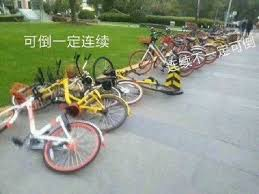
\includegraphics[width=0.94\textwidth,height=0.86\textheight,keepaspectratio]{assets/fig2.png}
\end{center}
\end{frame}

\section{几何与应用}

\begin{frame}{导数的几何意义}
过两点 $(x_0,f(x_0))$ 与 $(x,f(x))$ 的割线斜率为
\[
\frac{f(x)-f(x_0)}{x-x_0}.
\]
当 $x\to x_0$ 时，若极限存在，则得到切线斜率 $f'(x_0)$。

\vspace{0.6em}
因此切线方程为
\[
y=f'(x_0)(x-x_0)+f(x_0).
\]

若 $f'(x_0)\neq 0$，则法线方程为
\[
(x-x_0)+f'(x_0)(y-f(x_0))=0.
\]
\end{frame}

\begin{frame}[plain]{导数的几何直观}
\begin{center}
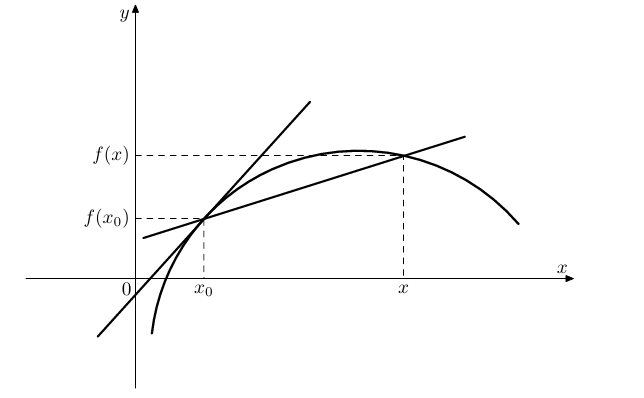
\includegraphics[width=0.92\textwidth,height=0.82\textheight,keepaspectratio]{assets/fig41.png}

\vspace{0.4em}

{\small 图 4.1\quad 导数与切线}
\end{center}
\end{frame}

\begin{frame}{导数与单调性}
\small
若函数 $f$ 在区间 $I$ 上可导，则
\begin{enumerate}
  \item 如果对任意 $x\in I$ 都有 $f'(x)>0$，则 $f$ 在 $I$ 上单调递增；
  \item 如果对任意 $x\in I$ 都有 $f'(x)<0$，则 $f$ 在 $I$ 上单调递减；
  \item 如果对任意 $x\in I$ 都有 $f'(x)=0$，则 $f$ 在 $I$ 上是常数函数。
\end{enumerate}

\vspace{0.5em}
\begin{block}{直观理解}
导数表示切线斜率。

当 $f'(x)>0$ 时，图像整体“向右上方走”，函数增大；当 $f'(x)<0$ 时，图像整体“向右下方走”，函数减小。
\end{block}
\end{frame}

\begin{frame}{单调性可视化}
\begin{center}
\begin{tikzpicture}[scale=0.92,>=Latex]
  \draw[->] (-0.2,0) -- (7.2,0) node[right] {$x$};
  \draw[->] (0,-0.3) -- (0,4.3) node[above] {$y$};
  \draw[thick,MainBlue,domain=0.4:2.2,samples=80] plot (\x,{0.45+0.65*(\x-0.5)});
  \draw[thick,MainBlue,domain=2.2:4.8,samples=80] plot (\x,{1.55+0.55*(\x-2.2)-0.20*(\x-3.5)^2});
  \draw[thick,MainBlue,domain=4.8:6.8,samples=80] plot (\x,{2.35-0.55*(\x-4.8)});
  \draw[dashed] (2.2,0)--(2.2,1.55);
  \draw[dashed] (4.8,0)--(4.8,2.35);
  \node at (1.2,3.6) {$f'(x)>0$};
  \node at (3.5,3.6) {$f'(x)=0$ 附近需判断};
  \node at (5.9,3.6) {$f'(x)<0$};
  \node[below] at (2.2,0) {$a$};
  \node[below] at (4.8,0) {$b$};
\end{tikzpicture}
\end{center}
\end{frame}

\begin{frame}{导数为 0 时如何判断}
\small
\textbf{要点：} 在某一个点上有 $f'(x_0)=0$，\alert{不能直接}得出“单增、单减、极大或极小”。

\vspace{0.4em}
需要看 $x_0$ 两侧导数符号是否发生变化：
\begin{enumerate}
  \item 若 $f'(x)$ 在 $x_0$ 左侧为负、右侧为正，则先减后增，$x_0$ 是极小值点；
  \item 若 $f'(x)$ 在 $x_0$ 左侧为正、右侧为负，则先增后减，$x_0$ 是极大值点；
  \item 若 $f'(x)$ 在 $x_0$ 两侧同号，则虽然 $f'(x_0)=0$，但通常不是极值点。
\end{enumerate}

\vspace{0.4em}
\textbf{典型例子：}
\begin{itemize}
  \item $f(x)=x^2$：$f'(0)=0$，且导数由负变正，所以 $x=0$ 是极小值点；
  \item $f(x)=x^3$：$f'(0)=0$，但导数在两侧都不改“增”的趋势，所以 $x=0$ 不是极值点；
  \item $f(x)\equiv C$：处处导数为 $0$，这时函数是常数。
\end{itemize}
\end{frame}

\begin{frame}{三种典型情形}
\begin{center}
\begin{tikzpicture}[scale=0.88,>=Latex]
  \begin{scope}[shift={(0,0)}]
    \draw[->] (-1.7,0) -- (1.7,0);
    \draw[->] (0,-0.2) -- (0,2.2);
    \draw[thick,MainBlue,domain=-1.35:1.35,samples=100] plot (\x,{0.55+0.7*\x*\x});
    \node at (0,-0.65) {\small $x^2$};
    \node at (0,-1.05) {\small 左负右正，极小};
  \end{scope}
  \begin{scope}[shift={(4.2,0)}]
    \draw[->] (-1.7,0) -- (1.7,0);
    \draw[->] (0,-0.2) -- (0,2.2);
    \draw[thick,MainBlue,domain=-1.35:1.35,samples=100] plot (\x,{1.95-0.7*\x*\x});
    \node at (0,-0.65) {\small $-x^2$};
    \node at (0,-1.05) {\small 左正右负，极大};
  \end{scope}
  \begin{scope}[shift={(8.4,0)}]
    \draw[->] (-1.7,0) -- (1.7,0);
    \draw[->] (0,-1.7) -- (0,1.9);
    \draw[thick,MainBlue,domain=-1.2:1.2,samples=100] plot (\x,{0.55*\x*\x*\x});
    \node at (0,-2.1) {\small $x^3$};
    \node at (0,-2.5) {\small 两侧同增，不是极值};
  \end{scope}
\end{tikzpicture}
\end{center}
\end{frame}

\section{运算法则}

\begin{frame}{线性法则与乘法法则}
设 $f,g$ 在 $x$ 处可导，$\alpha,\beta$ 为常数，则
\[
(\alpha f+\beta g)'=\alpha f'+\beta g',
\]
\[
(fg)'=f'g+fg'.
\]

\begin{block}{记忆}
和差逐项导，乘法交叉导。
\end{block}
\end{frame}

\begin{frame}{线性法则的证明}
\small
\textbf{答案：} 若 $f,g$ 在 $x$ 处可导，则
\[
f(x')=f(x)+f'(x)(x'-x)+o(x'-x),
\]
\[
g(x')=g(x)+g'(x)(x'-x)+o(x'-x).
\]
从而
\begin{align*}
\alpha f(x')+\beta g(x')
&=(\alpha f(x)+\beta g(x))+(\alpha f'(x)+\beta g'(x))(x'-x)\\
&\quad+\alpha o(x'-x)+\beta o(x'-x)\\
&=(\alpha f(x)+\beta g(x))+(\alpha f'(x)+\beta g'(x))(x'-x)+o(x'-x).
\end{align*}
这说明 $\alpha f+\beta g$ 在 $x$ 处可导，且
\[
(\alpha f+\beta g)'=\alpha f'+\beta g'.
\]
\end{frame}

\begin{frame}{乘法法则的证明}
\small
\textbf{答案：} 若 $f,g$ 在 $x$ 处可导，则 $f,g$ 在 $x$ 处连续，且
\[
f(x')g(x')=[f(x')-f(x)]g(x')+f(x)[g(x')-g(x)]+f(x)g(x).
\]
于是
\begin{align*}
\lim_{x'\to x}\frac{f(x')g(x')-f(x)g(x)}{x'-x}
&=\lim_{x'\to x}\frac{f(x')-f(x)}{x'-x}g(x')\\
&\quad+\lim_{x'\to x}\frac{g(x')-g(x)}{x'-x}f(x)\\
&=f'(x)g(x)+g'(x)f(x).
\end{align*}
因此 $fg$ 在 $x$ 处可导，且
\[
(fg)'=f'g+fg'.
\]
\end{frame}

\begin{frame}{商法则}
\small
\textbf{结论：} 设 $f,g$ 在 $x$ 处可导，且 $g(x)\neq 0$，则
\[
\left(\frac{f}{g}\right)'=\frac{f'g-fg'}{g^2}.
\]

\begin{block}{记忆}
上导下不导，减去上不导下导，再除以下平方。
\end{block}
\end{frame}

\begin{frame}{商法则的证明}
\small
\textbf{答案：} 先说明 $g^{-1}=\dfrac{1}{g}$ 在 $x$ 处可导：
\[
\lim_{x'\to x}\frac{g^{-1}(x')-g^{-1}(x)}{x'-x}
=\lim_{x'\to x}\frac{-1}{g(x)g(x')}\cdot\frac{g(x')-g(x)}{x'-x}
=-\frac{g'(x)}{g^2(x)}.
\]
因此 $\dfrac{f}{g}=f\cdot \dfrac{1}{g}$ 可导。由乘法法则得
\[
\left(\frac{f}{g}\right)'
=f'\cdot \frac{1}{g}+f\cdot \left(\frac{1}{g}\right)'
=\frac{f'g-fg'}{g^2}.
\]
\end{frame}

\begin{frame}{链式法则}
\small
\textbf{结论：} 设 $g$ 在 $x$ 处可导，$f$ 在 $g(x)$ 处可导，则复合函数 $f\circ g=f(g)$ 在 $x$ 处可导，且
\[
[f(g(x))]'=f'(g(x))g'(x).
\]
\end{frame}

\begin{frame}{链式法则结构图}
\begin{center}
\begin{tikzpicture}[>=Latex,node distance=1.7cm]
  \node[draw,rounded corners,fill=blue!8,minimum width=2.5cm,minimum height=0.95cm] (x) {$x$};
  \node[draw,rounded corners,fill=blue!8,minimum width=2.5cm,minimum height=0.95cm,right=of x] (g) {$u=g(x)$};
  \node[draw,rounded corners,fill=blue!8,minimum width=2.8cm,minimum height=0.95cm,right=of g] (f) {$y=f(u)=f(g(x))$};
  \draw[->,thick] (x) -- node[above] {$g'$} (g);
  \draw[->,thick] (g) -- node[above] {$f'$} (f);
  \node[below=1.1cm of g,align=center] {\small 先看外层，再乘内层\\[0.2em] \small $y'=f'(g(x))\cdot g'(x)$};
\end{tikzpicture}
\end{center}
\end{frame}

\begin{frame}{链式法则的证明}
\small
\textbf{答案：} 因为 $g$ 在 $x$ 处可导，故当 $x'\to x$ 时，
\[
g(x')=g(x)+g'(x)(x'-x)+o(x'-x).
\]
这说明存在常数 $C$，使得 $|g(x')-g(x)|\le C|x'-x|$。因此
\begin{align*}
f(g(x'))
&=f(g(x))+f'(g(x))(g(x')-g(x))+o(g(x')-g(x))\\
&=f(g(x))+f'(g(x))g'(x)(x'-x)+f'(g(x))o(x'-x)+o(x'-x)\\
&=f(g(x))+f'(g(x))g'(x)(x'-x)+o(x'-x).
\end{align*}
这说明 $f(g)$ 在 $x$ 处可导，且
\[
[f(g(x))]'=f'(g(x))g'(x).
\]
\end{frame}

\begin{frame}{反函数求导法则}
\small
\textbf{结论：} 设 $f$ 在 $x_0$ 附近连续且有反函数 $g$。如果 $f$ 在 $x_0$ 处可导，且 $f'(x_0)\neq 0$，令 $y_0=f(x_0)$，则 $g$ 在 $y_0$ 处可导，且
\[
g'(y_0)=\frac{1}{f'(x_0)}.
\]
\end{frame}

\begin{frame}{反函数求导可视化}
\begin{center}
\begin{tikzpicture}[scale=0.9,>=Latex]
  \draw[->] (-0.2,0) -- (5.8,0) node[right] {$x$};
  \draw[->] (0,-0.2) -- (0,5.6) node[above] {$y$};
  \draw[dashed,gray] (0,0) -- (5.2,5.2) node[above right] {$y=x$};
  \draw[thick,MainBlue,domain=0.6:4.6,samples=100] plot (\x,{0.55+0.72*\x+0.08*(\x-2.6)^2});
  \draw[thick,Accent,domain=0.6:4.6,samples=100] plot ({0.55+0.72*\x+0.08*(\x-2.6)^2},\x);
  \fill (2.0,{0.55+0.72*2.0+0.08*(2.0-2.6)^2}) circle (2pt) node[left] {\small $(x_0,y_0)$};
  \node[MainBlue] at (1.35,4.55) {\small $y=f(x)$};
  \node[Accent] at (4.45,1.2) {\small $x=g(y)$};
  \node[align=center] at (4.3,4.45) {\small 关于 $y=x$ 对称\\[-0.1em]\small 斜率互为倒数};
\end{tikzpicture}
\end{center}
\end{frame}

\begin{frame}{反函数求导的证明}
\small
\textbf{答案：} 因为 $f$ 在 $x_0$ 处可导，故
\[
f(x)=f(x_0)+f'(x_0)(x-x_0)+o(x-x_0)\qquad (x\to x_0).
\]
于是
\[
f(x)-f(x_0)=[f'(x_0)+o(1)](x-x_0).
\]
当 $f'(x_0)\neq 0$ 时，存在常数 $C>0$，使得
\[
|f(x)-f(x_0)|\ge C|x-x_0|.
\]
令 $y=f(x),\ y_0=f(x_0)$，又 $x=g(y)$，则当 $y\to y_0$ 时，$x=g(y)\to x_0$。代入上式得
\[
y-y_0=f'(x_0)(g(y)-g(y_0))+o(g(y)-g(y_0)).
\]
整理可写为
\[
g(y)=g(y_0)+\frac{1}{f'(x_0)}(y-y_0)+o(y-y_0).
\]
因此 $g$ 在 $y_0$ 处可导，且
\[
g'(y_0)=\frac{1}{f'(x_0)}.
\]
\end{frame}

\section{常用求导公式}

\begin{frame}{基本求导公式 I}
\small
\[
(C)'=0,\qquad (x)'=1,\qquad (\e^x)'=\e^x,
\]
\[
(x^\alpha)'=\alpha x^{\alpha-1},\qquad
(a^x)'=a^x\ln a,
\]
\[
(\ln|x|)'=\frac{1}{x},\qquad
(\log_a|x|)'=\frac{1}{x\ln a}.
\]

\vspace{0.6em}
\[
(\sin x)'=\cos x,\qquad
(\cos x)'=-\sin x,
\]
\[
(\tan x)'=\sec^2 x,\qquad
(\cot x)'=-\csc^2 x.
\]
\end{frame}

\begin{frame}{基本求导公式 II}
\small
\[
(\sec x)'=\sec x\tan x,\qquad
(\csc x)'=-\csc x\cot x.
\]
\[
(\arcsin x)'=\frac{1}{\sqrt{1-x^2}},\qquad
(\arccos x)'=-\frac{1}{\sqrt{1-x^2}}.
\]
\[
(\arctan x)'=\frac{1}{1+x^2},\qquad
(\operatorname{arccot}x)'=-\frac{1}{1+x^2}.
\]

\vspace{0.4em}
\[
(\sinh x)'=\cosh x,\qquad
(\cosh x)'=\sinh x,
\]
\[
(\tanh x)'=1-\tanh^2x,\qquad
(\coth x)'=1-\coth^2x.
\]
\end{frame}

\section{微分}

\begin{frame}{微分形式}
当 $f$ 可导时，
\[
\mathrm{d}f=f'(x)\dx.
\]

由求导法则可得
\[
\mathrm{d}(\alpha f+\beta g)=\alpha\,\mathrm{d}f+\beta\,\mathrm{d}g,
\]
\[
\mathrm{d}(fg)=g\,\mathrm{d}f+f\,\mathrm{d}g,
\]
\[
\mathrm{d}\!\left(\frac{f}{g}\right)=\frac{g\,\mathrm{d}f-f\,\mathrm{d}g}{g^2}.
\]

复合函数的形式不变性：
\[
\mathrm{d}[f(g)]=f'(g)\,\mathrm{d}g.
\]
\end{frame}

\section{例题}

\begin{frame}{例 1}
\small
\textbf{题目：} 求常值函数 $f(x)=c$ 的导数。
\end{frame}

\begin{frame}{例 1 的答案}
\small
\textbf{答案：} 设任意一点为 $x_0$，由导数定义，
\[
f'(x_0)=\lim_{x\to x_0}\frac{f(x)-f(x_0)}{x-x_0}.
\]
由于 $f(x)=c$ 是常值函数，所以
\[
f(x)-f(x_0)=c-c=0.
\]
因此
\[
f'(x_0)=\lim_{x\to x_0}\frac{0}{x-x_0}=0.
\]
这说明常值函数在任意点都可导，且
\[
(c)'=0.
\]
\end{frame}

\begin{frame}{例 2}
\small
\textbf{题目：} 研究函数 $f(x)=|x|$ 在 $x=0$ 处的可导性。
\end{frame}

\begin{frame}{例 2 的答案}
\small
\textbf{答案：} 先求左导数：
\[
f'_-(0)=\lim_{x\to 0^-}\frac{|x|-|0|}{x-0}
=\lim_{x\to 0^-}\frac{|x|}{x}.
\]
当 $x<0$ 时，$|x|=-x$，故
\[
f'_-(0)=\lim_{x\to 0^-}\frac{-x}{x}=-1.
\]
再求右导数：
\[
f'_+(0)=\lim_{x\to 0^+}\frac{|x|-|0|}{x-0}
=\lim_{x\to 0^+}\frac{|x|}{x}.
\]
当 $x>0$ 时，$|x|=x$，故
\[
f'_+(0)=\lim_{x\to 0^+}\frac{x}{x}=1.
\]
因为
\[
f'_-(0)\neq f'_+(0),
\]
所以 $f(x)=|x|$ 在 $x=0$ 处不可导。
\end{frame}

\begin{frame}{例 3}
\small
\textbf{题目：} 设
\[
f(x)=
\begin{cases}
\e^{-1/|x|}, & x\neq 0,\\
0, & x=0,
\end{cases}
\]
研究 $f$ 在 $x=0$ 处的可导性。
\end{frame}

\begin{frame}{例 3 的答案}
\small
\textbf{答案：} 由定义，
\[
f'(0)=\lim_{x\to 0}\frac{f(x)-f(0)}{x-0}
=\lim_{x\to 0}\frac{f(x)}{x}.
\]
先求右导数。当 $x>0$ 时，$|x|=x$，于是
\[
f'_+(0)=\lim_{x\to 0^+}\frac{\e^{-1/x}}{x}.
\]
令 $y=\frac{1}{x}$，则 $x\to 0^+$ 时，$y\to +\infty$，故
\[
f'_+(0)=\lim_{y\to +\infty}\frac{\e^{-y}}{1/y}
=\lim_{y\to +\infty}\frac{y}{\e^y}=0.
\]
同理，当 $x<0$ 时也有
\[
f'_-(0)=0.
\]
因此左右导数相等，所以 $f$ 在 $x=0$ 处可导，且
\[
f'(0)=0.
\]
\end{frame}

\begin{frame}{例 4}
\small
\textbf{题目：} 求函数
\[
f(x)=\ln\!\bigl(x+\sqrt{1+x^2}\bigr)
\]
的导数。
\end{frame}

\begin{frame}[allowframebreaks]{例 4 的答案}
\small
\textbf{答案：} 设
\[
u(x)=x+\sqrt{1+x^2},
\]
则
\[
f(x)=\ln u(x).
\]
由链式法则，
\[
f'(x)=\frac{u'(x)}{u(x)}.
\]
而
\[
u'(x)=1+\left(\sqrt{1+x^2}\right)'
=1+\frac{1}{2\sqrt{1+x^2}}\cdot 2x
=1+\frac{x}{\sqrt{1+x^2}}.
\]
代回得
\[
f'(x)=\frac{1+\dfrac{x}{\sqrt{1+x^2}}}{x+\sqrt{1+x^2}}.
\]
将分子通分：
\[
1+\frac{x}{\sqrt{1+x^2}}
=\frac{\sqrt{1+x^2}+x}{\sqrt{1+x^2}}.
\]
于是
\[
f'(x)=\frac{\sqrt{1+x^2}+x}{\sqrt{1+x^2}\,(x+\sqrt{1+x^2})}
=\frac{1}{\sqrt{1+x^2}}.
\]
\end{frame}

\begin{frame}{例 5}
\small
\textbf{题目：} 设 $u(x)>0$，$u(x),v(x)$ 都可导，求
\[
f(x)=u(x)^{v(x)}
\]
的导数。
\end{frame}

\begin{frame}{例 5 的答案}
\small
\textbf{答案：} 因为底数与指数都含变量，适合用对数求导。

先两边取对数：
\[
\ln f(x)=\ln\bigl(u(x)^{v(x)}\bigr)=v(x)\ln u(x).
\]
对两边求导，左边用链式法则，右边用乘法法则：
\[
\frac{f'(x)}{f(x)}=v'(x)\ln u(x)+v(x)\frac{u'(x)}{u(x)}.
\]
再乘回 $f(x)=u(x)^{v(x)}$，得到
\[
f'(x)=u(x)^{v(x)}
\left(v'(x)\ln u(x)+v(x)\frac{u'(x)}{u(x)}\right).
\]
\end{frame}

\begin{frame}{例 6}
\small
\textbf{题目：} 用微分法求
\[
f(x)=\ln\!\bigl(x^2\e^x+\sqrt{1+x^2}\bigr)
\]
的导数。
\end{frame}

\begin{frame}{例 6 的答案}
\small
\textbf{答案：} 由微分形式不变性，
\[
\mathrm{d}f=\bigl(x^2\e^x+\sqrt{1+x^2}\bigr)^{-1}
\mathrm{d}\!\bigl(x^2\e^x+\sqrt{1+x^2}\bigr).
\]
分别计算括号中两项的微分：
\[
\mathrm{d}(x^2\e^x)=x^2\,\mathrm{d}(\e^x)+\e^x\,\mathrm{d}(x^2)
=x^2\e^x\dx+2x\e^x\dx,
\]
\[
\mathrm{d}\!\bigl(\sqrt{1+x^2}\bigr)
=\frac{1}{2\sqrt{1+x^2}}\mathrm{d}(1+x^2)
=\frac{1}{2\sqrt{1+x^2}}\cdot 2x\dx
=\frac{x}{\sqrt{1+x^2}}\dx.
\]
所以
\[
\mathrm{d}f=
\frac{2x\e^x+x^2\e^x+\dfrac{x}{\sqrt{1+x^2}}}
{x^2\e^x+\sqrt{1+x^2}}\dx.
\]
从而
\[
f'(x)=
\frac{2x\e^x+x^2\e^x+\dfrac{x}{\sqrt{1+x^2}}}
{x^2\e^x+\sqrt{1+x^2}}.
\]
\end{frame}

\begin{frame}{例 7}
\small
\textbf{题目：} 由方程
\[
-y^2+2\e^y=x^2
\]
所确定的可微函数 $y=f(x)$，求 $\dfrac{\dy}{\dx}$。
\end{frame}

\begin{frame}{例 7 的答案}
\small
\textbf{答案：} 对方程两边关于 $x$ 求微分：
\[
\mathrm{d}(-y^2)+\mathrm{d}(2\e^y)=\mathrm{d}(x^2).
\]
分别计算各项：
\[
\mathrm{d}(-y^2)=-2y\dy,\qquad
\mathrm{d}(2\e^y)=2\e^y\dy,\qquad
\mathrm{d}(x^2)=2x\dx.
\]
故有
\[
-2y\dy+2\e^y\dy=2x\dx.
\]
整理得
\[
(2\e^y-2y)\dy=2x\dx.
\]
两边同时除以 $(2\e^y-2y)\dx$，便得到
\[
\frac{\dy}{\dx}=\frac{x}{\e^y-y}.
\]
\end{frame}
\section{课堂练习}

\begin{frame}{练习 1}
\footnotesize
设 $f(x)$ 在 $x_0$ 处可导，求极限
\[
\lim_{n\to\infty}n\left[f\left(x_0+\frac1n\right)-f(x_0)\right].
\]
\end{frame}

\begin{frame}{第 1 题答案}
\footnotesize
令
\[
h=\frac1n,
\]
则当 $n\to\infty$ 时，$h\to 0$。原极限可改写为
\[
\lim_{h\to0}\frac{f(x_0+h)-f(x_0)}{h}.
\]
这正是 $f$ 在 $x_0$ 处的导数定义，因此
\[
\lim_{n\to\infty}n\left[f\left(x_0+\frac1n\right)-f(x_0)\right]=f'(x_0).
\]
\end{frame}

\begin{frame}{练习 2}
\footnotesize
设 $f(x)$ 在 $x_0$ 处可导，求极限
\[
\lim_{h\to0}\frac{f(x_0+h)-f(x_0-h)}{h}.
\]
\end{frame}

\begin{frame}{第 2 题答案}
\footnotesize
把分子拆开：
\[
\frac{f(x_0+h)-f(x_0-h)}{h}
=\frac{f(x_0+h)-f(x_0)}{h}+\frac{f(x_0)-f(x_0-h)}{h}.
\]
第二项可改写为
\[
\frac{f(x_0)-f(x_0-h)}{h}=\frac{f(x_0-h)-f(x_0)}{-h}.
\]
于是当 $h\to0$ 时，前一项趋于 $f'(x_0)$，后一项也趋于 $f'(x_0)$，所以原极限为
\[
2f'(x_0).
\]
\end{frame}

\begin{frame}{练习 3}
\footnotesize
按照导数的定义求函数
\[
f(x)=x(x-1)^2(x-2)^2
\]
在 $x=0,1,2$ 处的导数。
\end{frame}

\begin{frame}{第 3 题答案}
\footnotesize
当 $x=0$ 时，$f(0)=0$，故
\[
f'(0)=\lim_{x\to0}\frac{x(x-1)^2(x-2)^2}{x}=\lim_{x\to0}(x-1)^2(x-2)^2=4.
\]
当 $x=1$ 时，$f(1)=0$，故
\[
f'(1)=\lim_{x\to1}\frac{x(x-1)^2(x-2)^2}{x-1}=\lim_{x\to1}x(x-1)(x-2)^2=0.
\]
当 $x=2$ 时，$f(2)=0$，故
\[
f'(2)=\lim_{x\to2}\frac{x(x-1)^2(x-2)^2}{x-2}=\lim_{x\to2}x(x-1)^2(x-2)=0.
\]
所以
\[
f'(0)=4,\qquad f'(1)=0,\qquad f'(2)=0.
\]
\end{frame}

\begin{frame}{练习 4}
\footnotesize
按照导数的定义求函数
\[
f(x)=\sqrt{1+x}
\]
在 $x=0,1,2$ 处的导数。
\end{frame}

\begin{frame}{第 4 题答案}
\footnotesize
在一般点 $x_0>-1$ 处，
\[
f'(x_0)=\lim_{x\to x_0}\frac{\sqrt{1+x}-\sqrt{1+x_0}}{x-x_0}.
\]
作有理化：
\[
f'(x_0)=\lim_{x\to x_0}\frac{(1+x)-(1+x_0)}{(x-x_0)(\sqrt{1+x}+\sqrt{1+x_0})}
=\lim_{x\to x_0}\frac{1}{\sqrt{1+x}+\sqrt{1+x_0}}.
\]
故
\[
f'(x_0)=\frac{1}{2\sqrt{1+x_0}}.
\]
于是
\[
f'(0)=\frac12,\qquad f'(1)=\frac{1}{2\sqrt2},\qquad f'(2)=\frac{1}{2\sqrt3}.
\]
\end{frame}

\begin{frame}{练习 5}
\footnotesize
设 $f(0)=0$，$f$ 在 $x=0$ 处可导，求极限
\[
\lim_{x\to0}\frac{f(x)}{x}.
\]
\end{frame}

\begin{frame}{第 5 题答案}
\footnotesize
由 $f(0)=0$，原式可写为
\[
\lim_{x\to0}\frac{f(x)-f(0)}{x-0}.
\]
因为 $f$ 在 $x=0$ 处可导，所以该极限等于 $f'(0)$，即
\[
\lim_{x\to0}\frac{f(x)}{x}=f'(0).
\]
\end{frame}

\begin{frame}{练习 6}
\footnotesize
已知函数 $f(x)=(x-a)\varphi(x)$，且 $\varphi(x)$ 为在 $a$ 处连续的函数，求 $f'(a)$。
\end{frame}

\begin{frame}{第 6 题答案}
\footnotesize
先算函数值：
\[
f(a)=(a-a)\varphi(a)=0.
\]
于是
\[
f'(a)=\lim_{x\to a}\frac{(x-a)\varphi(x)-0}{x-a}=\lim_{x\to a}\varphi(x).
\]
由于 $\varphi$ 在 $a$ 处连续，因此
\[
f'(a)=\varphi(a).
\]
\end{frame}

\begin{frame}{练习 7}
\footnotesize
证明函数
\[
f(x)=\begin{cases}
x^2,&x\text{ 为无理数},\\
0,&x\text{ 为有理数}
\end{cases}
\]
仅在 $x=0$ 处有导数。
\end{frame}

\begin{frame}{第 7 题答案}
\footnotesize
先考察 $x=0$。因为 $f(0)=0$，所以
\[
\frac{f(x)-f(0)}{x}=\begin{cases}
x,&x\text{ 为无理数},\\
0,&x\text{ 为有理数}.
\end{cases}
\]
当 $x\to0$ 时，上面两种情形都趋于 $0$，所以
\[
f'(0)=0.
\]

再考察 $x_0\neq0$。如果 $x_0$ 为有理数，则 $f(x_0)=0$，但可取无理数列 $x\to x_0$，此时 $f(x)=x^2\to x_0^2\neq0$，故 $f$ 在 $x_0$ 处不连续，从而不可导。

如果 $x_0$ 为无理数，则 $f(x_0)=x_0^2$，但可取有理数列 $x\to x_0$，此时 $f(x)=0\to0\neq x_0^2$，故在该点也不连续，从而不可导。

综上，函数仅在 $x=0$ 处有导数。
\end{frame}

\begin{frame}{练习 8}
\footnotesize
计算函数
\[
f(x)=\begin{cases}
x^2\sin\dfrac1x,&x\neq0,\\
0,&x=0
\end{cases}
\]
在 $x=0$ 处的导数。
\end{frame}

\begin{frame}{第 8 题答案}
\footnotesize
由定义
\[
f'(0)=\lim_{x\to0}\frac{x^2\sin(1/x)-0}{x}=\lim_{x\to0}x\sin\frac1x.
\]
因为
\[
-1\le\sin\frac1x\le1,
\]
故
\[
-|x|\le x\sin\frac1x\le |x|.
\]
当 $x\to0$ 时，两端都趋于 $0$，由夹逼定理得
\[
\lim_{x\to0}x\sin\frac1x=0.
\]
因此
\[
f'(0)=0.
\]
\end{frame}

\begin{frame}{练习 9}
\footnotesize
函数
\[
f(x)=\begin{cases}
x\sin\dfrac1x,&x\neq0,\\
0,&x=0
\end{cases}
\]
在 $x=0$ 处可导吗？
\end{frame}

\begin{frame}{第 9 题答案}
\footnotesize
由定义
\[
\frac{f(x)-f(0)}{x}=\sin\frac1x.
\]
如果 $f'(0)$ 存在，则极限
\[
\lim_{x\to0}\sin\frac1x
\]
必须存在。但取
\[
x_n=\frac{1}{\frac\pi2+2n\pi},\qquad y_n=\frac{1}{\frac{3\pi}{2}+2n\pi},
\]
则 $x_n\to0,\ y_n\to0$，且
\[
\sin\frac1{x_n}=1,\qquad \sin\frac1{y_n}=-1.
\]
两条收敛到 $0$ 的数列得到不同极限值，所以该极限不存在，故函数在 $x=0$ 处不可导。
\end{frame}

\begin{frame}{练习 10}
\footnotesize
确定常数 $a,b$ 的值，使得函数
\[
f(x)=\begin{cases}
x^2,&x\ge1,\\
ax+b,&x<1
\end{cases}
\]
在 $x=1$ 处可导。
\end{frame}

\begin{frame}{第 10 题答案}
\footnotesize
在 $x=1$ 处可导，必须先连续。由连续性得
\[
a+b=1.
\]
又左导数为 $a$，右导数为 $2$，故必须有
\[
a=2.
\]
代入 $a+b=1$ 得
\[
b=-1.
\]
因此
\[
a=2,\qquad b=-1.
\]
\end{frame}

\begin{frame}{练习 11}
\scriptsize
求下列函数的导数：
\begin{enumerate}
\setcounter{enumi}{10}
\item
\begin{enumerate}
\item $f(x)=2x^3+4x^2-3$；
\item $f(x)=(x+1)^2(x+2)(x+3)^3$；
\item $f(x)=(1+nx^m)(1+mx^n)$；
\item $f(x)=(ax^m+b)^n(cx^n+d)^m$；
\item $f(x)=x\sqrt{1+x^2}$；
\item $f(x)=\ln(\sin x)+e^{-x}\sin x$.
\end{enumerate}
\end{enumerate}
\end{frame}

\begin{frame}{第 11 题答案（1）--（2）}
\scriptsize
\textbf{(1)} 对多项式逐项求导：
\[
(2x^3)'=6x^2,\qquad (4x^2)'=8x,\qquad (-3)'=0.
\]
因此
\[
f'(x)=6x^2+8x.
\]

\textbf{(2)} 设
\[
f(x)=(x+1)^2(x+2)(x+3)^3.
\]
这类幂乘积直接展开比较麻烦，取对数更方便：
\[
\ln f(x)=2\ln(x+1)+\ln(x+2)+3\ln(x+3).
\]
两边对 $x$ 求导，得
\[
\frac{f'(x)}{f(x)}=\frac{2}{x+1}+\frac{1}{x+2}+\frac{3}{x+3}.
\]
再乘回 $f(x)$，得
\[
f'(x)=(x+1)^2(x+2)(x+3)^3
\left(\frac{2}{x+1}+\frac{1}{x+2}+\frac{3}{x+3}\right).
\]
\end{frame}

\begin{frame}{第 11 题答案（3）--（4）}
\scriptsize
\textbf{(3)} 设
\[
u(x)=1+nx^m,\qquad v(x)=1+mx^n.
\]
则
\[
u'(x)=mnx^{m-1},\qquad v'(x)=mnx^{n-1}.
\]
由乘法法则
\[
f'(x)=u'v+uv',
\]
所以
\[
f'(x)=mnx^{m-1}(1+mx^n)+mnx^{n-1}(1+nx^m).
\]

\textbf{(4)} 设
\[
f(x)=(ax^m+b)^n(cx^n+d)^m.
\]
仍用对数求导：
\[
\ln f(x)=n\ln(ax^m+b)+m\ln(cx^n+d).
\]
两边求导，得
\[
\frac{f'(x)}{f(x)}
=n\cdot\frac{amx^{m-1}}{ax^m+b}
+m\cdot\frac{cnx^{n-1}}{cx^n+d}.
\]
于是
\[
f'(x)=(ax^m+b)^n(cx^n+d)^m
\left(\frac{amnx^{m-1}}{ax^m+b}+\frac{cmnx^{n-1}}{cx^n+d}\right).
\]
\end{frame}

\begin{frame}{第 11 题答案（5）--（6）}
\scriptsize
\textbf{(5)} 设
\[
f(x)=x\sqrt{1+x^2}.
\]
由乘法法则，
\[
f'(x)=1\cdot\sqrt{1+x^2}+x\cdot(\sqrt{1+x^2})'.
\]
又因为
\[
(\sqrt{1+x^2})'=\frac{1}{2\sqrt{1+x^2}}\cdot 2x=\frac{x}{\sqrt{1+x^2}},
\]
所以
\[
f'(x)=\sqrt{1+x^2}+x\cdot\frac{x}{\sqrt{1+x^2}}
=\frac{1+2x^2}{\sqrt{1+x^2}}.
\]

\textbf{(6)} 设
\[
f(x)=\ln(\sin x)+e^{-x}\sin x.
\]
第一项由复合函数求导得
\[
(\ln(\sin x))'=\frac{\cos x}{\sin x}=\cot x.
\]
第二项用乘法法则：
\[
(e^{-x}\sin x)'=(e^{-x})'\sin x+e^{-x}(\sin x)'
=-e^{-x}\sin x+e^{-x}\cos x.
\]
故
\[
f'(x)=\cot x+e^{-x}(\cos x-\sin x).
\]
\end{frame}

\begin{frame}{练习 12}
\scriptsize
求下列函数的导数：
\begin{enumerate}
\setcounter{enumi}{11}
\item
\begin{enumerate}
\item $f(x)=\sqrt{\sin^2 x}$；
\item $f(x)=\dfrac{2+\sin x}{x}$；
\item $f(x)=\dfrac{x\ln x}{1+x}-\dfrac1x$；
\item $f(x)=\dfrac{\sin x}{1+\tan x}$；
\item $f(x)=\dfrac{xe^x-1}{\sin x}$；
\item $f(x)=\dfrac{x^2}{(1-x)^2(1+x)}$；
\item $f(x)=\ln\!\dfrac{1-x^2}{1+x^2}$；
\item $f(x)=\dfrac{x^p(1-x)^q}{1+x}$；
\item $f(x)=\dfrac{x\sin x+\cos x}{x\sin x-\cos x}$.
\end{enumerate}
\end{enumerate}
\end{frame}

\begin{frame}[allowframebreaks]{第 12 题答案（1）--（3）}
\scriptsize
\textbf{(1)} 因为
\[
\sqrt{\sin^2x}=|\sin x|,
\]
所以可分段写成
\[
f(x)=
\begin{cases}
\sin x,& \sin x>0,\\
-\sin x,& \sin x<0.
\end{cases}
\]
当 $\sin x\neq0$ 时，
\[
f'(x)=\operatorname{sgn}(\sin x)\cos x.
\]
在 $x=k\pi$ 处，$|\sin x|$ 的左右导数不相等，因此这些点不可导。

\textbf{(2)} 设
\[
f(x)=\frac{2+\sin x}{x}.
\]
由商法则，
\[
f'(x)=\frac{x\cos x-(2+\sin x)}{x^2}.
\]

\textbf{(3)} 设
\[
f(x)=\frac{x\ln x}{1+x}-\frac1x.
\]
先求第一项的导数。设
\[
u=x\ln x,\qquad v=1+x,
\]
则
\[
u'=\ln x+1,\qquad v'=1.
\]
由商法则，
\[
\left(\frac{x\ln x}{1+x}\right)'=
\frac{(\ln x+1)(1+x)-x\ln x}{(1+x)^2}
=\frac{\ln x+1+x}{(1+x)^2}.
\]
又
\[
\left(-\frac1x\right)'=\frac1{x^2},
\]
所以
\[
f'(x)=\frac{\ln x+1+x}{(1+x)^2}+\frac{1}{x^2}.
\]
\end{frame}

\begin{frame}[allowframebreaks]{第 12 题答案（4）--（6）}
\scriptsize
\textbf{(4)} 原式先化简：
\[
\frac{\sin x}{1+\tan x}
=\frac{\sin x}{1+\frac{\sin x}{\cos x}}
=\frac{\sin x\cos x}{\sin x+\cos x}.
\]
设
\[
u=\sin x\cos x,\qquad v=\sin x+\cos x.
\]
则
\[
u'=\cos^2x-\sin^2x,\qquad v'=\cos x-\sin x.
\]
由商法则，
\[
f'(x)=\frac{u'v-uv'}{v^2}.
\]
代入并整理得
\[
f'(x)=\frac{\cos^3x-\sin^3x}{(\sin x+\cos x)^2}.
\]

\textbf{(5)} 设
\[
f(x)=\frac{xe^x-1}{\sin x}.
\]
分子导数为
\[
(xe^x-1)'=e^x+xe^x.
\]
由商法则，
\[
f'(x)=\frac{(e^x+xe^x)\sin x-(xe^x-1)\cos x}{\sin^2x}.
\]

\textbf{(6)} 设
\[
f(x)=\frac{x^2}{(1-x)^2(1+x)}.
\]
这题适合用对数求导：
\[
\ln f(x)=2\ln x-2\ln(1-x)-\ln(1+x).
\]
两边求导，得
\[
\frac{f'(x)}{f(x)}=\frac2x+\frac{2}{1-x}-\frac1{1+x}.
\]
因此
\[
f'(x)=\frac{x^2}{(1-x)^2(1+x)}
\left(\frac2x+\frac{2}{1-x}-\frac1{1+x}\right).
\]
\end{frame}

\begin{frame}[allowframebreaks]{第 12 题答案（7）--（9）}
\scriptsize
\textbf{(7)} 设
\[
f(x)=\ln\!\frac{1-x^2}{1+x^2}=\ln(1-x^2)-\ln(1+x^2).
\]
逐项求导：
\[
f'(x)=\frac{-2x}{1-x^2}-\frac{2x}{1+x^2}
=-\frac{4x}{1-x^4}.
\]

\textbf{(8)} 设
\[
f(x)=\frac{x^p(1-x)^q}{1+x}.
\]
对数求导：
\[
\ln f(x)=p\ln x+q\ln(1-x)-\ln(1+x).
\]
两边求导得
\[
\frac{f'(x)}{f(x)}=\frac{p}{x}-\frac{q}{1-x}-\frac1{1+x}.
\]
故
\[
f'(x)=\frac{x^p(1-x)^q}{1+x}
\left(\frac{p}{x}-\frac{q}{1-x}-\frac1{1+x}\right).
\]

\textbf{(9)} 设
\[
u=x\sin x+\cos x,\qquad v=x\sin x-\cos x.
\]
则
\[
u'=x\cos x,
\qquad
v'=x\cos x+2\sin x.
\]
由商法则，
\[
f'(x)=\frac{u'v-uv'}{v^2}.
\]
代入并整理得
\[
f'(x)=-\frac{2x+\sin2x}{(x\sin x-\cos x)^2}.
\]
\end{frame}

\begin{frame}{练习 13}
\scriptsize
求下列函数的导数：
\begin{enumerate}
\setcounter{enumi}{12}
\item
\begin{enumerate}
\item $f(x)=e^{x^2\sin x}$；
\item $f(x)=\dfrac{x}{\sqrt{a^2+x^2}}$；
\item $f(x)=\arcsin(\cos^2x)$；
\item $f(x)=\dfrac{\arcsin x}{\sqrt{1-x^2}}$；
\item $f(x)=\ln(\ln(\ln x))$；
\item $f(x)=\ln(\sin x+\cos x)$；
\item $f(x)=\sqrt{x+\sqrt x}$；
\item $f(x)=e^{\alpha x}\sin\beta x$；
\item $f(x)=\sin(\sin(\cos x))$.
\end{enumerate}
\end{enumerate}
\end{frame}

\begin{frame}[allowframebreaks]{第 13 题答案（1）--（3）}
\scriptsize
\textbf{(1)} 设
\[
f(x)=e^{x^2\sin x}.
\]
由复合函数求导，
\[
f'(x)=e^{x^2\sin x}\cdot (x^2\sin x)'.
\]
而
\[
(x^2\sin x)'=2x\sin x+x^2\cos x,
\]
所以
\[
f'(x)=e^{x^2\sin x}(2x\sin x+x^2\cos x).
\]

\textbf{(2)} 设
\[
f(x)=\frac{x}{\sqrt{a^2+x^2}}=x(a^2+x^2)^{-1/2}.
\]
由乘法法则，
\[
f'(x)=(a^2+x^2)^{-1/2}+x\cdot\left(-\frac12\right)(a^2+x^2)^{-3/2}\cdot 2x.
\]
即
\[
f'(x)=\frac{1}{\sqrt{a^2+x^2}}-\frac{x^2}{(a^2+x^2)^{3/2}}
=\frac{a^2}{(a^2+x^2)^{3/2}}.
\]

\textbf{(3)} 设
\[
f(x)=\arcsin(\cos^2x).
\]
由链式法则，
\[
f'(x)=\frac{1}{\sqrt{1-\cos^4x}}\cdot (\cos^2x)'.
\]
又
\[
(\cos^2x)'=2\cos x(-\sin x)=-2\sin x\cos x,
\]
故
\[
f'(x)=\frac{-2\sin x\cos x}{\sqrt{1-\cos^4x}}.
\]
\end{frame}

\begin{frame}[allowframebreaks]{第 13 题答案（4）--（6）}
\scriptsize
\textbf{(4)} 设
\[
f(x)=\frac{\arcsin x}{\sqrt{1-x^2}}.
\]
取
\[
u=\arcsin x,\qquad v=(1-x^2)^{-1/2}.
\]
则
\[
u'=\frac1{\sqrt{1-x^2}},\qquad
v'=\frac{x}{(1-x^2)^{3/2}}.
\]
所以
\[
f'(x)=u'v+uv'
=\frac{1}{1-x^2}+\frac{x\arcsin x}{(1-x^2)^{3/2}}.
\]

\textbf{(5)} 三重复合函数逐层求导：
\[
f(x)=\ln(\ln(\ln x)).
\]
于是
\[
f'(x)=\frac1{\ln(\ln x)}\cdot\frac1{\ln x}\cdot\frac1x
=\frac{1}{x\ln x\ln(\ln x)}.
\]

\textbf{(6)} 设
\[
f(x)=\ln(\sin x+\cos x).
\]
由链式法则，
\[
f'(x)=\frac{\cos x-\sin x}{\sin x+\cos x}.
\]
\end{frame}

\begin{frame}[allowframebreaks]{第 13 题答案（7）--（9）}
\scriptsize
\textbf{(7)} 设
\[
f(x)=\sqrt{x+\sqrt x}=(x+\sqrt x)^{1/2}.
\]
则
\[
f'(x)=\frac12(x+\sqrt x)^{-1/2}\left(1+\frac1{2\sqrt x}\right),
\]
即
\[
f'(x)=\frac{1+\frac{1}{2\sqrt x}}{2\sqrt{x+\sqrt x}}.
\]

\textbf{(8)} 设
\[
f(x)=e^{\alpha x}\sin\beta x.
\]
由乘法法则，
\[
f'(x)=(e^{\alpha x})'\sin\beta x+e^{\alpha x}(\sin\beta x)'.
\]
而
\[
(e^{\alpha x})'=\alpha e^{\alpha x},\qquad
(\sin\beta x)'=\beta\cos\beta x.
\]
所以
\[
f'(x)=e^{\alpha x}(\alpha\sin\beta x+\beta\cos\beta x).
\]

\textbf{(9)} 这是三层复合函数：
\[
f(x)=\sin(\sin(\cos x)).
\]
依次求导，
\[
f'(x)=\cos(\sin(\cos x))\cdot (\sin(\cos x))',
\]
\[
(\sin(\cos x))'=\cos(\cos x)(-\sin x).
\]
于是
\[
f'(x)=-\sin x\cos(\cos x)\cos(\sin(\cos x)).
\]
\end{frame}

\begin{frame}{练习 14}
\scriptsize
求下列函数的导数：
\begin{enumerate}
\setcounter{enumi}{13}
\item
\begin{enumerate}
\item $f(x)=(x\sin x)^x$；
\item $f(x)=x^{a^x}$；
\item $f(x)=(\cos x)^{\sin x}+(\sin x)^{\cos x}$；
\item $f(x)=x\sqrt{\dfrac{1-x}{1+x}}$；
\item $f(x)=a^{x^n}$；
\item $f(x)=(x+\sqrt{1+x^2})^n$.
\end{enumerate}
\end{enumerate}
\end{frame}

\begin{frame}[allowframebreaks]{第 14 题答案（1）--（2）}
\scriptsize
\textbf{(1)} 取对数：
\[
\ln f=x\ln(x\sin x).
\]
两边求导：
\[
\frac{f'}{f}=\ln(x\sin x)+x\cdot\frac{(x\sin x)'}{x\sin x}.
\]
而
\[
(x\sin x)'=\sin x+x\cos x,
\]
所以
\[
\frac{(x\sin x)'}{x\sin x}
=\frac{\sin x+x\cos x}{x\sin x}
=\frac1x+\cot x.
\]
因此
\[
f'(x)=(x\sin x)^x[\ln(x\sin x)+1+x\cot x].
\]

\textbf{(2)} 设
\[
f(x)=x^{a^x}.
\]
取对数：
\[
\ln f=a^x\ln x,
\]
两边求导得
\[
\frac{f'}{f}=a^x\ln a\cdot \ln x+a^x\cdot\frac1x.
\]
所以
\[
f'(x)=x^{a^x}a^x\left(\ln a\,\ln x+\frac1x\right).
\]
\end{frame}

\begin{frame}[allowframebreaks]{第 14 题答案（3）--（4）}
\scriptsize
\textbf{(3)} 原函数是两项之和：
\[
f(x)=(\cos x)^{\sin x}+(\sin x)^{\cos x}.
\]
先对第一项
\[
y_1=(\cos x)^{\sin x}
\]
取对数：
\[
\ln y_1=\sin x\ln(\cos x).
\]
求导得
\[
\frac{y_1'}{y_1}=\cos x\ln(\cos x)+\sin x\cdot\frac{-\sin x}{\cos x}.
\]
于是
\[
y_1'=(\cos x)^{\sin x}\left(\cos x\ln(\cos x)-\frac{\sin^2x}{\cos x}\right).
\]
再对第二项
\[
y_2=(\sin x)^{\cos x}
\]
取对数：
\[
\ln y_2=\cos x\ln(\sin x).
\]
求导得
\[
\frac{y_2'}{y_2}=-\sin x\ln(\sin x)+\cos x\cdot\frac{\cos x}{\sin x}.
\]
所以
\[
y_2'=(\sin x)^{\cos x}\left(-\sin x\ln(\sin x)+\frac{\cos^2x}{\sin x}\right).
\]
因此 $f'(x)=y_1'+y_2'$。

\textbf{(4)} 设
\[
f(x)=x\sqrt{\frac{1-x}{1+x}}.
\]
由乘法法则，
\[
f'(x)=\sqrt{\frac{1-x}{1+x}}+x\left(\sqrt{\frac{1-x}{1+x}}\right)'.
\]
对根式部分用链式法则并整理，可得
\[
f'(x)=\sqrt{\frac{1-x}{1+x}}\left(1-\frac{x}{1-x^2}\right).
\]
\end{frame}

\begin{frame}[allowframebreaks]{第 14 题答案（5）--（6）}
\scriptsize
\textbf{(5)} 设
\[
f(x)=a^{x^n}.
\]
这是指数函数与幂函数的复合。由链式法则，
\[
f'(x)=a^{x^n}\ln a\cdot (x^n)'.
\]
而
\[
(x^n)'=nx^{n-1},
\]
所以
\[
f'(x)=a^{x^n}\ln a\cdot nx^{n-1}.
\]

\textbf{(6)} 设
\[
f(x)=(x+\sqrt{1+x^2})^n.
\]
由链式法则，
\[
f'(x)=n(x+\sqrt{1+x^2})^{n-1}\left(1+\frac{x}{\sqrt{1+x^2}}\right).
\]
把括号中的因子通分：
\[
1+\frac{x}{\sqrt{1+x^2}}
=\frac{x+\sqrt{1+x^2}}{\sqrt{1+x^2}}.
\]
于是
\[
f'(x)=n(x+\sqrt{1+x^2})^{n-1}
\cdot\frac{x+\sqrt{1+x^2}}{\sqrt{1+x^2}}
=\frac{n(x+\sqrt{1+x^2})^n}{\sqrt{1+x^2}}.
\]
\end{frame}

\begin{frame}{练习 15}
\scriptsize
设 $f(x)$ 可导，求 $y'$：
\begin{enumerate}
\setcounter{enumi}{14}
\item
\begin{enumerate}
\item $y=f(x\sin x)$；
\item $y=f(e^x)e^{f(x)}$；
\item $y=f(\cos x)\sin x$；
\item $y=f(f(f(x)))$；
\item $y=f(\tan x)$；
\item $y=[f(\ln x)]^n$.
\end{enumerate}
\end{enumerate}
\end{frame}

\begin{frame}[allowframebreaks]{第 15 题答案（1）--（3）}
\scriptsize
\textbf{(1)} 设
\[
y=f(x\sin x).
\]
由链式法则，
\[
y'=f'(x\sin x)\cdot (x\sin x)'.
\]
而
\[
(x\sin x)'=\sin x+x\cos x,
\]
故
\[
y'=f'(x\sin x)(\sin x+x\cos x).
\]

\textbf{(2)} 设
\[
y=f(e^x)e^{f(x)}.
\]
由乘法法则，
\[
y'=[f(e^x)]'e^{f(x)}+f(e^x)[e^{f(x)}]'.
\]
再分别用链式法则：
\[
[f(e^x)]'=f'(e^x)\cdot e^x,
\]
\[
[e^{f(x)}]'=e^{f(x)}f'(x).
\]
代回得
\[
y'=e^{f(x)}\bigl[e^x f'(e^x)+f(e^x)f'(x)\bigr].
\]

\textbf{(3)} 设
\[
y=f(\cos x)\sin x.
\]
由乘法法则，
\[
y'=[f(\cos x)]'\sin x+f(\cos x)\cos x.
\]
又
\[
[f(\cos x)]'=f'(\cos x)(-\sin x),
\]
故
\[
y'=-f'(\cos x)\sin^2x+f(\cos x)\cos x.
\]
\end{frame}

\begin{frame}[allowframebreaks]{第 15 题答案（4）--（6）}
\scriptsize
\textbf{(4)} 设
\[
y=f(f(f(x))).
\]
这是三层复合函数，逐层求导：
\[
y'=f'(f(f(x)))\cdot [f(f(x))]'.
\]
而
\[
[f(f(x))]'=f'(f(x))f'(x),
\]
所以
\[
y'=f'(f(f(x)))f'(f(x))f'(x).
\]

\textbf{(5)} 设
\[
y=f(\tan x).
\]
由链式法则，
\[
y'=f'(\tan x)\sec^2x.
\]

\textbf{(6)} 设
\[
y=[f(\ln x)]^n.
\]
把外层看成幂函数，先对外层求导：
\[
y'=n[f(\ln x)]^{n-1}\cdot [f(\ln x)]'.
\]
再对内层求导：
\[
[f(\ln x)]'=f'(\ln x)\cdot \frac1x.
\]
因此
\[
y'=n[f(\ln x)]^{n-1}f'(\ln x)\frac1x.
\]
\end{frame}

\begin{frame}{练习 16}
\scriptsize
设 $u(x),v(x)$ 可导，求 $y'$：
\begin{enumerate}
\setcounter{enumi}{15}
\item
\begin{enumerate}
\item $y=\sqrt{u^2+v^2}$；
\item $y=\arctan\dfrac{u}{v}$；
\item $y=\sqrt[v]{u}$；
\item $y=\dfrac{u}{v^2}$；
\item $y=\dfrac{1}{\sqrt{u^2+v^2}}$；
\item $y=ue^v$.
\end{enumerate}
\end{enumerate}
\end{frame}

\begin{frame}[allowframebreaks]{第 16 题答案（1）--（3）}
\scriptsize
\textbf{(1)} 设
\[
y=\sqrt{u^2+v^2}=(u^2+v^2)^{1/2}.
\]
由链式法则，
\[
y'=\frac12(u^2+v^2)^{-1/2}(2uu'+2vv').
\]
化简得
\[
y'=\frac{uu'+vv'}{\sqrt{u^2+v^2}}.
\]

\textbf{(2)} 设
\[
y=\arctan\frac{u}{v}.
\]
先设
\[
t=\frac{u}{v},
\]
则
\[
y'=\frac{t'}{1+t^2}.
\]
而
\[
t'=\frac{u'v-uv'}{v^2},
\qquad
1+t^2=1+\frac{u^2}{v^2}=\frac{u^2+v^2}{v^2}.
\]
所以
\[
y'=\frac{u'v-uv'}{u^2+v^2}.
\]

\textbf{(3)} 设
\[
y=\sqrt[v]{u}=u^{1/v}.
\]
这题适合用对数求导。取对数得
\[
\ln y=\frac{1}{v}\ln u,
\]
两边求导：
\[
\frac{y'}{y}=\left(\frac1v\right)'\ln u+\frac1v\cdot\frac{u'}u
=-\frac{v'}{v^2}\ln u+\frac{u'}{uv}.
\]
因此
\[
y'=u^{1/v}\left(\frac{u'}{uv}-\frac{v'\ln u}{v^2}\right).
\]
\end{frame}

\begin{frame}[allowframebreaks]{第 16 题答案（4）--（6）}
\scriptsize
\textbf{(4)} 设
\[
y=\frac{u}{v^2}=u\,v^{-2}.
\]
由乘法法则，
\[
y'=u'v^{-2}+u(-2)v^{-3}v'
=\frac{u'v-2uv'}{v^3}.
\]

\textbf{(5)} 设
\[
y=\frac{1}{\sqrt{u^2+v^2}}=(u^2+v^2)^{-1/2}.
\]
由链式法则，
\[
y'=-\frac12(u^2+v^2)^{-3/2}(2uu'+2vv').
\]
所以
\[
y'=-\frac{uu'+vv'}{(u^2+v^2)^{3/2}}.
\]

\textbf{(6)} 设
\[
y=ue^v.
\]
由乘法法则，
\[
y'=u'e^v+u(e^v)'.
\]
又
\[
(e^v)'=e^vv',
\]
所以
\[
y'=e^v(u'+uv').
\]
\end{frame}

\begin{frame}{练习 17}
\footnotesize
通过对 $(1+x)^n$ 求导并利用二项式定理证明
\[
\sum_{k=0}^n kC_n^k=n2^{n-1},\qquad
\sum_{k=0}^n k^2C_n^k=n(n+1)2^{n-2}.
\]
\end{frame}

\begin{frame}[allowframebreaks]{第 17 题答案}
\footnotesize
由二项式定理
\[
(1+x)^n=\sum_{k=0}^n C_n^k x^k.
\]
求导得
\[
n(1+x)^{n-1}=\sum_{k=1}^n kC_n^k x^{k-1}.
\]
令 $x=1$，得
\[
\sum_{k=0}^n kC_n^k=n2^{n-1}.
\]
再求一次导数：
\[
n(n-1)(1+x)^{n-2}=\sum_{k=2}^n k(k-1)C_n^k x^{k-2}.
\]
令 $x=1$，得
\[
\sum_{k=0}^n k(k-1)C_n^k=n(n-1)2^{n-2}.
\]
再利用
\[
k^2=k(k-1)+k,
\]
可得
\[
\sum_{k=0}^n k^2C_n^k=n(n+1)2^{n-2}.
\]
\end{frame}

\begin{frame}{练习 18}
\footnotesize
证明：可导偶函数的导数为奇函数，可导奇函数的导数为偶函数，可导周期函数的导数仍为周期函数。
\end{frame}

\begin{frame}{第 18 题答案}
\footnotesize
若 $f$ 为偶函数，则 $f(-x)=f(x)$。两边求导得
\[
-f'(-x)=f'(x),
\]
所以 $f'(-x)=-f'(x)$，即 $f'$ 为奇函数。

若 $f$ 为奇函数，则 $f(-x)=-f(x)$。两边求导得
\[
-f'(-x)=-f'(x),
\]
所以 $f'(-x)=f'(x)$，即 $f'$ 为偶函数。

若 $f(x+T)=f(x)$，两边求导得
\[
f'(x+T)=f'(x),
\]
所以 $f'$ 仍以 $T$ 为周期。
\end{frame}

\begin{frame}{练习 19}
\footnotesize
$(*)$ 设 $a_{ij}(x)$ 均为可导函数，求行列式函数 $\det(a_{ij}(x))_{n\times n}$ 的导数。
\end{frame}

\begin{frame}{第 19 题答案}
\footnotesize
设
\[
D(x)=\det(a_{ij}(x))_{n\times n}.
\]
由行列式对每一行的线性性，保留一阶项即可得
\[
D'(x)=\sum_{r=1}^n
\det\begin{pmatrix}
 a_{11}(x)&\cdots&a_{1n}(x)\\
 \vdots&&\vdots\\
 a'_{r1}(x)&\cdots&a'_{rn}(x)\\
 \vdots&&\vdots\\
 a_{n1}(x)&\cdots&a_{nn}(x)
\end{pmatrix}.
\]
即逐行求导后分别成行列式，再求和。
\end{frame}

\begin{frame}{练习 20}
\footnotesize
$(*)$ 设 Riemann 函数定义为
\[
R(x)=\begin{cases}
\dfrac1p,&x=\dfrac qp\in(0,1)\cap\mathbb Q,\ q,p\text{ 互素},\\
0,&x\in(0,1)\setminus\mathbb Q.
\end{cases}
\]
讨论其可导性。
\end{frame}

\begin{frame}[allowframebreaks]{第 20 题答案}
\footnotesize
这就是 Thomae 函数。在每一个有理点 $x_0=\dfrac{q}{p}$ 处，
\[
R(x_0)=\frac1p>0,
\]
而在任意邻域内都存在无理数 $x$ 使 $R(x)=0$，所以在有理点不连续，从而不可导。

至于无理点，虽然函数连续，但导数问题比较细致，不属于本节常规求导法则的直接应用范围。因此在本讲义中，只要求掌握：它在每一个有理点都不可导；更深入的无理点可导性属于拓展内容。
\end{frame}

\section{高阶导数}

\begin{frame}{高阶导数的定义}
\small
如果函数 $f$ 在 $x_0$ 附近可导，并且导函数 $f'$ 在 $x_0$ 处仍可导，就称 $f$ 在 $x_0$ 处二阶可导，记
\[
f''(x_0)=(f')'(x_0).
\]

一般地，若 $f^{(n)}$ 在 $x_0$ 处可导，则称 $f$ 在 $x_0$ 处 $n+1$ 阶可导，并记
\[
f^{(n+1)}(x_0)=\bigl(f^{(n)}\bigr)'(x_0).
\]

\vspace{0.5em}
常见记号：
\[
f^{(1)}=f',\quad f^{(2)}=f'',\quad f^{(3)}=f''',
\]
\[
f''=\frac{\mathrm d^2f}{\mathrm dx^2},\qquad
f'''=\frac{\mathrm d^3f}{\mathrm dx^3}.
\]
\end{frame}

\begin{frame}{例题：线性函数的二阶导数}
\small
\textbf{题目：} 求线性函数
\[
f(x)=ax+b
\]
的二阶导数。
\end{frame}

\begin{frame}{线性函数的二阶导数答案}
\small
先对 $f(x)=ax+b$ 求一阶导数：
\[
f'(x)=(ax+b)'=a.
\]
再求一次导数：
\[
f''(x)=(a)'=0.
\]
因此线性函数的二阶导数恒为零，即
\[
f''(x)=0.
\]
这也对应于匀速直线运动的加速度为零。
\end{frame}

\begin{frame}{例题：二次函数的二阶导数}
\small
\textbf{题目：} 求二次函数
\[
f(x)=x^2
\]
的二阶导数。
\end{frame}

\begin{frame}{二次函数的二阶导数答案}
\small
先求一阶导数：
\[
f'(x)=(x^2)'=2x.
\]
再求二阶导数：
\[
f''(x)=(2x)'=2.
\]
因此
\[
f''(x)=2.
\]
这说明二次函数的二阶导数是常数。
\end{frame}

\begin{frame}{区间上的高阶可导与连续可导}
\small
如果 $f$ 在区间 $I$ 的每一点处都 $n$ 阶可导，则称 $f$ 在 $I$ 中 $n$ 阶可导。

\vspace{0.5em}
如果 $f$ 可导且 $f'$ 连续，则称 $f$ 为一阶连续可导函数，记作
\[
f\in C^1(I).
\]

一般地，如果 $f$ 在 $I$ 中 $n$ 阶可导，且 $f^{(n)}$ 连续，则称 $f\in C^n(I)$。

\vspace{0.5em}
如果 $f$ 在 $I$ 中存在任意阶导数，则称 $f$ 为\alert{光滑函数}，记作
\[
f\in C^\infty(I).
\]
\end{frame}

\begin{frame}{例题：可微函数的导数不一定连续}
\small
\textbf{题目：} 分析函数
\[
f(x)=
\begin{cases}
x^{\frac32}\sin\dfrac1x,&x\in(0,1],\\
0,&x=0
\end{cases}
\]
的导数连续性。
\end{frame}

\begin{frame}[allowframebreaks]{导数不连续的例子答案}
\small
先求 $x=0$ 处的导数。由定义
\[
f'(0)=\lim_{x\to0^+}\frac{x^{3/2}\sin(1/x)-0}{x}
=\lim_{x\to0^+}\sqrt{x}\sin\frac1x.
\]
由于
\[
\left|\sqrt{x}\sin\frac1x\right|\le \sqrt{x}\to0,
\]
所以
\[
f'(0)=0.
\]

当 $x>0$ 时，由乘法法则与链式法则，
\[
f'(x)=\left(x^{3/2}\right)'\sin\frac1x+x^{3/2}\left(\sin\frac1x\right)'
\]
\[
=\frac32x^{1/2}\sin\frac1x+x^{3/2}\cos\frac1x\left(-\frac1{x^2}\right)
\]
\[
=\frac32x^{1/2}\sin\frac1x-x^{-1/2}\cos\frac1x.
\]
取
\[
x_n=\frac1{2n\pi}\qquad (n=1,2,\dots),
\]
则
\[
\cos\frac1{x_n}=\cos(2n\pi)=1,
\]
于是
\[
f'(x_n)=\frac32x_n^{1/2}\sin(2n\pi)-x_n^{-1/2}
=-x_n^{-1/2}\to-\infty.
\]
因此 $f'$ 在 $x=0$ 附近无界，从而 $f'$ 在 $x=0$ 处不连续。这个例子说明：\alert{可微函数的导数不一定连续}。
\end{frame}

\begin{frame}{例题：$C^k$ 但不是 $C^{k+1}$ 的函数}
\small
\textbf{题目：} 设 $k=1,2,\dots$，讨论函数
\[
f(x)=
\begin{cases}
x^{2k+1}\sin\dfrac1x,&x\ne0,\\
0,&x=0
\end{cases}
\]
的可导阶数。
\end{frame}

\begin{frame}[allowframebreaks]{$C^k$ 但不是 $C^{k+1}$ 的函数答案}
\small
与前一个例子的思路类似，先在 $x=0$ 处用定义求导，可以得到
\[
f'(0)=0.
\]
对 $x\ne0$ 时逐次求导，会不断出现两类项：一类是高次幂乘以 $\sin(1/x)$，另一类是较低次幂乘以 $\cos(1/x)$。

\vspace{0.4em}
例如
\[
f'(x)=(2k+1)x^{2k}\sin\frac1x-x^{2k-1}\cos\frac1x\qquad (x\ne0),
\]
继续求导可见，直到求到第 $k$ 阶时，仍然可以写成
\[
f^{(k)}(x)=x^2\phi(x)\pm x\sin\frac1x
\]
或
\[
f^{(k)}(x)=x^2\phi(x)\pm x\cos\frac1x,
\]
其中 $\phi(x)$ 在 $x=0$ 附近有界。

因此
\[
f^{(k)}(x)\to0\qquad (x\to0),
\]
从而 $f^{(k)}$ 在 $x=0$ 处连续，故 $f\in C^k$。

\vspace{0.4em}
但再多求一次导数时，会出现不再被 $x$ 压住的振荡项，如 $\sin(1/x)$ 或 $\cos(1/x)$ 本身，因此 $f^{(k+1)}$ 在 $x=0$ 处不存在或不连续。故该函数是
\[
C^k\ \text{函数，但不是}\ C^{k+1}\ \text{函数}.
\]
\end{frame}

\begin{frame}{例题：光滑但非解析型的经典函数}
\small
\textbf{题目：} 分析函数
\[
f(x)=
\begin{cases}
0,&x\le0,\\
e^{-1/x},&x>0
\end{cases}
\]
的高阶可导性质。
\end{frame}

\begin{frame}[allowframebreaks]{光滑函数例子答案}
\small
先看 $x=0$ 处的一阶导数。因为 $f(0)=0$，所以
\[
f'_+(0)=\lim_{x\to0^+}\frac{e^{-1/x}}{x}.
\]
令 $t=\frac1x$，则 $t\to+\infty$，于是
\[
f'_+(0)=\lim_{t\to+\infty}\frac{te^{-t}}{1}=0.
\]
左侧本来就是常值零函数，所以 $f'(0)=0$。

\vspace{0.4em}
当 $x>0$ 时，
\[
f'(x)=e^{-1/x}\cdot\frac1{x^2}.
\]
继续求导可以发现：每求一次导，都会得到“关于 $1/x$ 的多项式”乘上 $e^{-1/x}$。也就是说存在多项式 $p_k$，使得
\[
f^{(k)}(x)=
\begin{cases}
0,&x\le0,\\
p_k(1/x)e^{-1/x},&x>0.
\end{cases}
\]

由于指数衰减 $e^{-1/x}$ 比任意幂次 $x^{-m}$ 的增长都更快地趋于零，所以对任意 $k$，
\[
\lim_{x\to0^+}p_k(1/x)e^{-1/x}=0.
\]
于是
\[
f^{(k)}(0)=0
\]
对任意 $k$ 都成立。

因此该函数在 $x=0$ 处存在任意阶导数，并且在整个定义域上是光滑的，即
\[
f\in C^\infty.
\]
\end{frame}

\begin{frame}{高阶导数的运算法则}
\small
\textbf{结论：} 设 $f,g$ 均为 $n$ 阶可导函数，则
\begin{enumerate}
  \item $(\alpha f+\beta g)^{(n)}=\alpha f^{(n)}+\beta g^{(n)}$；
  \item \textbf{Leibniz 公式}
  \[
  (fg)^{(n)}=\sum_{k=0}^n C_n^k f^{(n-k)}g^{(k)}.
  \]
\end{enumerate}
\end{frame}

\begin{frame}[allowframebreaks]{高阶乘积求导公式的证明}
\small
\textbf{(1)} 线性公式可以由一阶求导的线性性反复使用，直接用归纳法得到。

\vspace{0.4em}
\textbf{(2)} 对 $n$ 用数学归纳法。

当 $n=1$ 时，
\[
(fg)'=f'g+fg',
\]
命题成立。

假设对 $n=k$ 时成立，即
\[
(fg)^{(k)}=\sum_{l=0}^k C_k^l f^{(k-l)}g^{(l)}.
\]
则对 $n=k+1$，
\[
(fg)^{(k+1)}=\left[(fg)^{(k)}\right]'
=\sum_{l=0}^k C_k^l\left[f^{(k-l+1)}g^{(l)}+f^{(k-l)}g^{(l+1)}\right].
\]
把同类项合并，并利用组合恒等式
\[
C_k^l+C_k^{l-1}=C_{k+1}^l,
\]
便得到
\[
(fg)^{(k+1)}=\sum_{l=0}^{k+1} C_{k+1}^l f^{(k+1-l)}g^{(l)}.
\]
归纳完成。
\end{frame}

\begin{frame}{例题：多项式的高阶导数}
\small
\textbf{题目：} 设
\[
p_n(x)=a_nx^n+a_{n-1}x^{n-1}+\cdots+a_1x+a_0
\]
是 $n$ 次多项式。求它的高阶导数，并说明如何由导数恢复系数。
\end{frame}

\begin{frame}{多项式高阶导数答案}
\small
对多项式逐项求导即可。每求一次导，最高次幂下降一阶，并带出一个系数。连续求 $k$ 次后，
\[
p_n^{(k)}(x)
=n(n-1)\cdots(n-k+1)a_nx^{n-k}+\cdots+k!a_k.
\]

于是当 $k=n$ 时，只剩最高次项贡献，因此
\[
p_n^{(n)}(x)=n!a_n.
\]
若再继续求导，则导数恒为零，所以
\[
p_n^{(k)}(x)=0\qquad (k>n).
\]

另外令 $x=0$，就得到
\[
p_n^{(k)}(0)=k!a_k,
\]
从而
\[
a_k=\frac1{k!}p_n^{(k)}(0),\qquad k=0,1,\dots,n.
\]
这说明多项式在 $0$ 点各阶导数完全决定了它的系数。
\end{frame}

\begin{frame}{例题：指数函数的各阶导数}
\small
\textbf{题目：} 求函数
\[
f(x)=a^x
\]
的各阶导数。
\end{frame}

\begin{frame}{指数函数各阶导数答案}
\small
先求一阶导数：
\[
f'(x)=a^x\ln a.
\]
再求一次：
\[
f''(x)=(a^x\ln a)'=a^x(\ln a)^2.
\]
继续下去，每求一次导数都会再乘一个 $\ln a$，因此可以归纳得到
\[
f^{(n)}(x)=a^x(\ln a)^n.
\]
这就是指数函数高阶导数的通项公式。
\end{frame}

\begin{frame}{例题：$\sin x,\cos x$ 的各阶导数}
\small
\textbf{题目：} 求函数 $\sin x$ 与 $\cos x$ 的各阶导数。
\end{frame}

\begin{frame}{三角函数各阶导数答案}
\small
先列出前几阶导数：
\[
(\sin x)'=\cos x=\sin\left(x+\frac{\pi}{2}\right),
\]
\[
(\sin x)''=-\sin x=\sin(x+\pi),
\]
\[
(\sin x)'''=-\cos x=\sin\left(x+\frac{3\pi}{2}\right).
\]
可以看出每求一次导数，相位都向前平移 $\dfrac{\pi}{2}$，因此
\[
(\sin x)^{(n)}=\sin\left(x+\frac{n\pi}{2}\right).
\]

同理，
\[
(\cos x)'=-\sin x=\cos\left(x+\frac{\pi}{2}\right),
\]
从而
\[
(\cos x)^{(n)}=\cos\left(x+\frac{n\pi}{2}\right).
\]
\end{frame}

\begin{frame}{例题：有理函数的各阶导数}
\small
\textbf{题目：} 求函数
\[
\frac{1}{1-x},\qquad \frac{1}{2-3x+x^2}
\]
的各阶导数。
\end{frame}

\begin{frame}{有理函数各阶导数答案}
\small
先看
\[
f(x)=\frac{1}{1-x}=(1-x)^{-1}.
\]
前几次求导为
\[
f'(x)=\frac{1}{(1-x)^2},\qquad
f''(x)=\frac{2}{(1-x)^3}.
\]
继续观察可归纳得
\[
f^{(n)}(x)=\frac{n!}{(1-x)^{n+1}}.
\]

再看
\[
\frac{1}{2-3x+x^2}=\frac{1}{(1-x)(2-x)}
=\frac{1}{1-x}-\frac{1}{2-x}.
\]
因此
\[
\left(\frac{1}{2-3x+x^2}\right)^{(n)}
=\frac{n!}{(1-x)^{n+1}}-\frac{n!}{(2-x)^{n+1}}.
\]
这里的关键是先裂项，再分别对简单分式求高阶导数。
\end{frame}

\begin{frame}{例题：$\arctan x$ 的高阶导数}
\small
\textbf{题目：} 设
\[
f(x)=\arctan x,
\]
试分析 $f^{(n)}(x)$ 的形式。
\end{frame}

\begin{frame}[allowframebreaks]{$\arctan x$ 高阶导数答案}
\small
设
\[
y=\arctan x,
\]
则
\[
x=\tan y.
\]
于是
\[
y'=\frac1{1+x^2}=\cos^2 y.
\]
又因为
\[
\cos^2 y=\cos y\cdot \cos y=\cos y\sin\left(y+\frac{\pi}{2}\right),
\]
继续求导可以发现，高阶导数始终可以写成
\[
y^{(n)}=(n-1)!\cos^n y\cdot \sin\left(ny+\frac{n\pi}{2}\right)
\]
这一类形式。

\vspace{0.4em}
把 $y=\arctan x$ 代回，就得到 $f^{(n)}(x)$ 的显式结构。这里重点不在死记公式，而在于掌握：\alert{把反三角函数先设成隐变量，再利用三角恒等变形寻找归纳模式}。
\end{frame}

\begin{frame}{例题：复合函数的三阶导数}
\small
\textbf{题目：} 设 $f,g$ 均为三阶可导函数，求复合函数 $f(g(x))$ 的三阶导数。
\end{frame}

\begin{frame}{复合函数三阶导数答案}
\small
先由链式法则求一阶导数：
\[
[f(g)]'=f'(g)g'.
\]
再求二阶导数：
\[
[f(g)]''=[f'(g)g']'=f''(g)(g')^2+f'(g)g''.
\]
继续求三阶导数：
\[
[f(g)]'''
=\left[f''(g)(g')^2+f'(g)g''\right]'.
\]
分别求导：
\[
\left[f''(g)(g')^2\right]'=f^{(3)}(g)(g')^3+2f''(g)g'g'',
\]
\[
\left[f'(g)g''\right]'=f''(g)g'g''+f'(g)g^{(3)}.
\]
相加得
\[
[f(g)]^{(3)}=f^{(3)}(g)(g')^3+3f''(g)g'g''+f'(g)g^{(3)}.
\]
这也是更一般高阶复合求导公式的低阶原型。
\end{frame}

\section{高阶导数练习}

\begin{frame}{高阶导数练习 1}
\small
求下列函数指定阶的导数：
\begin{enumerate}
\item $f(x)=e^x\cos x$，求 $f^{(5)}$；
\item $f(x)=x^2\ln x+x\ln^2x$，求 $f''$；
\item $f(x)=x^2e^x$，求 $f^{(10)}$；
\item $f(x)=x^5\cos x$，求 $f^{(50)}$；
\item $f(x)=(x^2+1)\cosh x$，求 $f^{(10)}$；
\item $f(x)=x\sinh x$，求 $f^{(100)}$。
\end{enumerate}
\end{frame}

\begin{frame}[allowframebreaks]{高阶导数练习 1 答案}
\small
\textbf{(1)} 先连续求导：
\[
f'(x)=e^x(\cos x-\sin x),\quad
f''(x)=-2e^x\sin x,
\]
\[
f^{(3)}(x)=-2e^x(\sin x+\cos x),\quad
f^{(4)}(x)=-4e^x\cos x.
\]
故
\[
f^{(5)}(x)=\bigl(-4e^x\cos x\bigr)'=-4e^x(\cos x-\sin x)=4e^x(\sin x-\cos x).
\]

\textbf{(2)}
\[
f'(x)=2x\ln x+x+\ln^2x+2\ln x,
\]
\[
f''(x)=2\ln x+2+1+\frac{2\ln x}{x}+\frac2x
=2\ln x+3+\frac{2\ln x+2}{x}.
\]

\textbf{(3)} 对 $x^2e^x$ 可归纳得
\[
(x^2e^x)^{(n)}=e^x\bigl(x^2+2nx+n(n-1)\bigr),
\]
所以
\[
f^{(10)}(x)=e^x(x^2+20x+90).
\]

\textbf{(4)} 用 Leibniz 公式：
\[
f^{(50)}=\sum_{k=0}^5 C_{50}^k (x^5)^{(k)}(\cos x)^{(50-k)}.
\]
代入各项并利用 $\cos x$ 的导数循环，可得
\[
f^{(50)}=-x^5\cos x-250x^4\sin x+24500x^3\cos x
\]
\[
+1176000x^2\sin x-27636000x\cos x-254251200\sin x.
\]

\textbf{(5)}
\[
f^{(10)}=\sum_{k=0}^2 C_{10}^k (x^2+1)^{(k)}(\cosh x)^{(10-k)}.
\]
由于 $\cosh x$ 的偶阶导仍为 $\cosh x$，奇阶导为 $\sinh x$，于是
\[
f^{(10)}=(x^2+1)\cosh x+20x\sinh x+90\cosh x,
\]
即
\[
f^{(10)}=(x^2+91)\cosh x+20x\sinh x.
\]

\textbf{(6)} 同理，
\[
f^{(100)}=x\sinh x+100\cosh x.
\]
\end{frame}

\begin{frame}{高阶导数练习 2}
\small
求下列函数的 $n$ 阶导数：
\begin{enumerate}
\item $f(x)=\dfrac{ax+b}{cx+d}$；
\item $f(x)=\sin ax\sin bx$；
\item $f(x)=\dfrac{\ln x}{x}$；
\item $f(x)=x\ln x$；
\item $f(x)=\dfrac{x^n}{1+x}$；
\item $f(x)=x^ne^{ax}$；
\item $f(x)=\dfrac1{x^2-2x-8}$；
\item $f(x)=x\cos ax$；
\item $f(x)=\dfrac{e^x}{x}$。
\end{enumerate}
\end{frame}

\begin{frame}[allowframebreaks]{高阶导数练习 2 答案}
\small
\textbf{(1)} 先裂项：
\[
\frac{ax+b}{cx+d}=\frac ac+\frac{bc-ad}{c(cx+d)}.
\]
常数项高阶导为零，而
\[
\left(\frac1{cx+d}\right)^{(n)}=\frac{(-1)^nn!c^n}{(cx+d)^{n+1}}.
\]
故
\[
f^{(n)}(x)=(-1)^{n-1}\frac{n!c^{n-1}(ad-bc)}{(cx+d)^{n+1}}.
\]

\textbf{(2)} 用积化和差：
\[
\sin ax\sin bx=\frac12\bigl[\cos(a-b)x-\cos(a+b)x\bigr].
\]
于是
\[
f^{(n)}(x)=\frac12\Bigl[(a-b)^n\cos\!\left((a-b)x+\frac{n\pi}{2}\right)
-(a+b)^n\cos\!\left((a+b)x+\frac{n\pi}{2}\right)\Bigr].
\]

\textbf{(3)} 可归纳得到
\[
\left(\frac{\ln x}{x}\right)^{(n)}
=(-1)^n\frac{n!}{x^{n+1}}\bigl(\ln x-H_n\bigr),
\]
其中
\[
H_n=1+\frac12+\cdots+\frac1n.
\]

\textbf{(4)} 当 $n=1$ 时，
\[
(x\ln x)'=\ln x+1.
\]
当 $n\ge2$ 时，
\[
(x\ln x)^{(n)}=(-1)^n\frac{(n-2)!}{x^{n-1}}.
\]

\textbf{(5)} 先做整除：
\[
\frac{x^n}{1+x}=x^{n-1}-x^{n-2}+\cdots+(-1)^{n-1}+(-1)^n\frac1{1+x}.
\]
前面多项式的 $n$ 阶导数为零，所以
\[
f^{(n)}(x)=(-1)^n\left(\frac1{1+x}\right)^{(n)}=\frac{n!}{(1+x)^{n+1}}.
\]
\end{frame}

\begin{frame}[allowframebreaks]{高阶导数练习 2 答案（续）}
\small
\textbf{(6)} 对 $x^ne^{ax}$ 用 Leibniz 公式：
\[
f^{(n)}(x)=\sum_{k=0}^n C_n^k (x^n)^{(k)}(e^{ax})^{(n-k)}.
\]
而
\[
(x^n)^{(k)}=\frac{n!}{(n-k)!}x^{n-k},\qquad (e^{ax})^{(n-k)}=a^{n-k}e^{ax},
\]
故
\[
f^{(n)}(x)=e^{ax}\sum_{k=0}^n C_n^k \frac{n!}{(n-k)!}a^{n-k}x^{n-k}.
\]

\textbf{(7)} 先裂项：
\[
\frac1{x^2-2x-8}=\frac1{(x-4)(x+2)}=\frac16\left(\frac1{x-4}-\frac1{x+2}\right).
\]
因此
\[
f^{(n)}(x)=\frac{(-1)^nn!}{6}\left[\frac1{(x-4)^{n+1}}-\frac1{(x+2)^{n+1}}\right].
\]

\textbf{(8)} 用 Leibniz 公式，因为 $x$ 的二阶及以上导数全为零，
\[
f^{(n)}(x)=x(\cos ax)^{(n)}+n(\cos ax)^{(n-1)}.
\]
于是
\[
f^{(n)}(x)=xa^n\cos\!\left(ax+\frac{n\pi}{2}\right)
+na^{n-1}\cos\!\left(ax+\frac{(n-1)\pi}{2}\right).
\]

\textbf{(9)}
\[
f^{(n)}(x)=\sum_{k=0}^n C_n^k (e^x)^{(n-k)}\left(\frac1x\right)^{(k)}
=e^x\sum_{k=0}^n C_n^k (-1)^k\frac{k!}{x^{k+1}}.
\]
\end{frame}

\begin{frame}{高阶导数练习 3}
\small
证明下列等式：
\begin{enumerate}
\item $(\ln x)^{(n)}=\dfrac{(-1)^{n-1}(n-1)!}{x^n}$，$n\ge1$；
\item $(\sin^4x+\cos^4x)^{(n)}=4^{n-1}\cos\!\left(4x+\dfrac{n\pi}{2}\right)$，$n\ge1$；
\item $(e^{ax}\sin bx)^{(n)}=(a^2+b^2)^{n/2}e^{ax}\sin(bx+n\varphi)$，其中
\[
\sin\varphi=\frac{b}{\sqrt{a^2+b^2}},\qquad
\cos\varphi=\frac{a}{\sqrt{a^2+b^2}}.
\]
\end{enumerate}
\end{frame}

\begin{frame}[allowframebreaks]{高阶导数练习 3 答案}
\small
\textbf{(1)} 用归纳法。$n=1$ 时显然成立。若对 $n=k$ 成立，即
\[
(\ln x)^{(k)}=\frac{(-1)^{k-1}(k-1)!}{x^k},
\]
则
\[
(\ln x)^{(k+1)}=\left[\frac{(-1)^{k-1}(k-1)!}{x^k}\right]'
=(-1)^k\frac{k!}{x^{k+1}}.
\]
所以结论对一切 $n\ge1$ 成立。

\textbf{(2)} 先化简：
\[
\sin^4x+\cos^4x
=(\sin^2x+\cos^2x)^2-2\sin^2x\cos^2x
=1-\frac12\sin^22x
=\frac34+\frac14\cos4x.
\]
常数项高阶导为零，所以
\[
(\sin^4x+\cos^4x)^{(n)}
=\frac14(\cos4x)^{(n)}
=4^{n-1}\cos\left(4x+\frac{n\pi}{2}\right).
\]

\textbf{(3)} 设
\[
r=\sqrt{a^2+b^2},
\]
并取角 $\varphi$ 满足
\[
a=r\cos\varphi,\qquad b=r\sin\varphi.
\]
则
\[
e^{ax}\sin bx=\Im\bigl(e^{(a+ib)x}\bigr).
\]
而
\[
(a+ib)^n=r^n(\cos n\varphi+i\sin n\varphi),
\]
所以
\[
\frac{\mathrm d^n}{\mathrm dx^n}\bigl(e^{(a+ib)x}\bigr)=(a+ib)^ne^{(a+ib)x}
=r^ne^{ax}e^{ibx}(\cos n\varphi+i\sin n\varphi).
\]
取虚部即可得到
\[
(e^{ax}\sin bx)^{(n)}=r^ne^{ax}\sin(bx+n\varphi).
\]
\end{frame}

\begin{frame}{高阶导数练习 4}
\small
\textbf{题目：} 求函数
\[
f(x)=\sqrt{1+x}
\]
的各阶导数。
\end{frame}

\begin{frame}{高阶导数练习 4 答案}
\small
把函数写成幂函数形式：
\[
f(x)=(1+x)^{1/2}.
\]
连续求导可以发现：
\[
f'(x)=\frac12(1+x)^{-1/2},
\]
\[
f''(x)=-\frac1{2^2}(1+x)^{-3/2},
\]
\[
f^{(3)}(x)=\frac{1\cdot3}{2^3}(1+x)^{-5/2}.
\]
于是归纳得到
\[
f^{(n)}(x)=\frac{\left(\frac12\right)\left(\frac12-1\right)\cdots\left(\frac12-n+1\right)}{(1+x)^{n-\frac12}}.
\]
也可写成更紧凑的形式：
\[
f^{(n)}(x)=(-1)^{n-1}\frac{(2n-3)!!}{2^n}(1+x)^{-n+\frac12}\qquad (n\ge1).
\]
\end{frame}

\begin{frame}{高阶导数练习 5}
\small
\textbf{题目：} 求函数
\[
f(x)=e^x\cos x
\]
的各阶导数。
\end{frame}

\begin{frame}{高阶导数练习 5 答案}
\small
由前面的计算可知，
\[
f'(x)=e^x(\cos x-\sin x),
\]
\[
f''(x)=-2e^x\sin x,
\]
继续求导会发现每次求导都相当于把相位平移 $\dfrac{\pi}{4}$，并把振幅乘上 $\sqrt2$。因此
\[
f^{(n)}(x)=2^{n/2}e^x\cos\left(x+\frac{n\pi}{4}\right).
\]
这个公式也可以由复数方法
\[
e^x\cos x=\Re\bigl(e^{(1+i)x}\bigr)
\]
迅速得到。
\end{frame}

\begin{frame}{高阶导数练习 6}
\small
设 $f$ 的各阶导数都存在，求下列函数的二阶导数与三阶导数：
\begin{enumerate}
\item $y=f(x^3)$；
\item $y=f(e^{-x})$；
\item $y=f(f(x))$；
\item $y=f(\ln x)$。
\end{enumerate}
\end{frame}

\begin{frame}[allowframebreaks]{高阶导数练习 6 答案}
\small
\textbf{(1)} 设 $u=x^3$，则
\[
y'=f'(u)\cdot 3x^2.
\]
再求导得
\[
y''=f''(u)(3x^2)^2+f'(u)\cdot6x=9x^4f''(u)+6xf'(u).
\]
再求一次，
\[
y'''=27x^6f'''(u)+54x^3f''(u)+6f'(u).
\]

\textbf{(2)} 设 $u=e^{-x}$，则 $u'=-u$。于是
\[
y'=-uf'(u).
\]
再求导：
\[
y''=u f'(u)+u^2f''(u).
\]
再求一次：
\[
y'''=-u f'(u)-3u^2f''(u)-u^3f'''(u).
\]
\end{frame}

\begin{frame}[allowframebreaks]{高阶导数练习 6 答案（续）}
\small
\textbf{(3)} 设 $u=f(x)$，则
\[
y'=f'(u)f'(x).
\]
再求导：
\[
y''=f''(u)\bigl(f'(x)\bigr)^2+f'(u)f''(x).
\]
继续求导：
\[
y'''=f'''(u)\bigl(f'(x)\bigr)^3+3f''(u)f'(x)f''(x)+f'(u)f'''(x).
\]

\textbf{(4)} 设 $u=\ln x$，则
\[
y'=\frac{f'(u)}{x}.
\]
再求导：
\[
y''=\frac{f''(u)-f'(u)}{x^2}.
\]
再求一次：
\[
y'''=\frac{f'''(u)-3f''(u)+2f'(u)}{x^3}.
\]
\end{frame}

\begin{frame}{高阶导数练习 7}
\small
\textbf{题目：} 验证函数
\[
y=e^x\sin x
\]
满足方程
\[
y''-2y'+2y=0.
\]
\end{frame}

\begin{frame}{高阶导数练习 7 答案}
\small
先求导：
\[
y'=e^x(\sin x+\cos x),
\]
\[
y''=e^x(\sin x+\cos x)+e^x(\cos x-\sin x)=2e^x\cos x.
\]
代入左端：
\[
y''-2y'+2y
=2e^x\cos x-2e^x(\sin x+\cos x)+2e^x\sin x=0.
\]
因此该函数满足所给微分方程。
\end{frame}

\begin{frame}{高阶导数练习 8}
\small
\textbf{题目：} 验证函数
\[
y=a\sin(\alpha x+\varphi)+b\cos(\alpha x+\varphi)
\]
满足方程
\[
y''+\alpha^2y=0.
\]
\end{frame}

\begin{frame}{高阶导数练习 8 答案}
\small
先求一阶导数：
\[
y'=a\alpha\cos(\alpha x+\varphi)-b\alpha\sin(\alpha x+\varphi).
\]
再求一次：
\[
y''=-a\alpha^2\sin(\alpha x+\varphi)-b\alpha^2\cos(\alpha x+\varphi).
\]
于是
\[
y''=-\alpha^2\bigl[a\sin(\alpha x+\varphi)+b\cos(\alpha x+\varphi)\bigr]
=-\alpha^2y.
\]
所以
\[
y''+\alpha^2y=0.
\]
\end{frame}

\begin{frame}{高阶导数练习 9}
\small
\textbf{题目：} 验证函数
\[
y=ae^{\alpha x}+be^{\beta x}
\]
满足方程
\[
y''-(\alpha+\beta)y'+\alpha\beta y=0.
\]
\end{frame}

\begin{frame}{高阶导数练习 9 答案}
\small
先求导：
\[
y'=a\alpha e^{\alpha x}+b\beta e^{\beta x},
\]
\[
y''=a\alpha^2 e^{\alpha x}+b\beta^2 e^{\beta x}.
\]
代入原式左端：
\[
y''-(\alpha+\beta)y'+\alpha\beta y
\]
\[
=a\bigl[\alpha^2-(\alpha+\beta)\alpha+\alpha\beta\bigr]e^{\alpha x}
+b\bigl[\beta^2-(\alpha+\beta)\beta+\alpha\beta\bigr]e^{\beta x}.
\]
两个括号都等于零，因此整个式子恒为零。
\end{frame}

\begin{frame}{高阶导数练习 10}
\small
\textbf{题目：} 验证函数
\[
y=\arcsin x
\]
满足方程
\[
xy'=(1-x^2)y''
\]
并求 $y^{(n)}(0)$。
\end{frame}

\begin{frame}[allowframebreaks]{高阶导数练习 10 答案}
\small
先求导：
\[
y'=\frac1{\sqrt{1-x^2}},
\]
\[
y''=\frac{x}{(1-x^2)^{3/2}}.
\]
因此
\[
(1-x^2)y''=(1-x^2)\cdot\frac{x}{(1-x^2)^{3/2}}
=\frac{x}{\sqrt{1-x^2}}=xy'.
\]
方程成立。

再利用级数展开
\[
\arcsin x=\sum_{m=0}^{\infty}\frac{(2m)!}{4^m(m!)^2(2m+1)}x^{2m+1},
\]
于是偶次导数在 $0$ 处全为零：
\[
y^{(2m)}(0)=0.
\]
而奇次导数满足
\[
y^{(2m+1)}(0)=(2m+1)!\cdot \frac{(2m)!}{4^m(m!)^2(2m+1)}
=\frac{[(2m)!]^2}{4^m(m!)^2}.
\]
所以
\[
y^{(2m)}(0)=0,\qquad
y^{(2m+1)}(0)=\frac{[(2m)!]^2}{4^m(m!)^2}.
\]
\end{frame}

\begin{frame}{高阶导数练习 11}
\small
\textbf{题目：} 通过对 $(1-x)^n$ 求导并利用二项式定理证明
\[
\sum_{k=0}^n(-1)^kC_n^kk^m=
\begin{cases}
0,&m=0,1,\dots,n-1,\\
(-1)^nn!,&m=n.
\end{cases}
\]
\end{frame}

\begin{frame}[allowframebreaks]{高阶导数练习 11 答案}
\small
由二项式定理，
\[
(1-x)^n=\sum_{k=0}^n(-1)^kC_n^kx^k.
\]
对两边求 $m$ 次导数，得
\[
\frac{\mathrm d^m}{\mathrm dx^m}(1-x)^n
=\sum_{k=0}^n(-1)^kC_n^k\,k(k-1)\cdots(k-m+1)x^{k-m}.
\]

令 $x=1$。当 $m<n$ 时，左边是
\[
(-1)^m n(n-1)\cdots(n-m+1)(1-x)^{n-m}\Big|_{x=1}=0.
\]
因此右边也为零。再利用 $k^m$ 可以表示成若干个下降幂的线性组合，就得到
\[
\sum_{k=0}^n(-1)^kC_n^kk^m=0\qquad (m<n).
\]

当 $m=n$ 时，左边变成
\[
\frac{\mathrm d^n}{\mathrm dx^n}(1-x)^n=(-1)^nn!.
\]
右边在 $x=1$ 处正好对应
\[
\sum_{k=0}^n(-1)^kC_n^kk^n.
\]
于是
\[
\sum_{k=0}^n(-1)^kC_n^kk^n=(-1)^nn!.
\]
结论得证。
\end{frame}
\begin{frame}{总结}
\begin{enumerate}
  \item 可导的判定关键是差商极限，或左右导数是否相等。
  \item 可导等价于可微，本质是局部线性近似。
  \item 复合结构优先想链式法则，复杂幂式优先想对数求导。
  \item 微分法在隐函数求导和复杂表达式求导中尤其高效。
\end{enumerate}
\end{frame}

\end{document}
